\documentclass[11pt,letterpaper]{article}
\usepackage[T1]{fontenc}
\usepackage[utf8]{inputenc}
\usepackage{amsmath}
\usepackage{newtxtext,newtxmath}
\usepackage[margin=1in]{geometry}
\usepackage{microtype,parskip,graphicx,booktabs,array,float,caption,titlesec,textcomp}
\PassOptionsToPackage{hyphens}{url}
\usepackage[hidelinks]{hyperref}
\urlstyle{same}
\DeclareUnicodeCharacter{2212}{\textminus}
\captionsetup{font=small,labelfont=bf,labelsep=period,justification=raggedright,singlelinecheck=false,skip=4pt}
\titleformat*{\section}{\large\bfseries}
\titleformat*{\subsection}{\normalsize\bfseries\itshape}
\titlespacing*{\section}{0pt}{14pt}{4pt}
\titlespacing*{\subsection}{0pt}{10pt}{2pt}
\hypersetup{pdftitle={Is the Naive Hedge Still Hard to Beat?},pdfauthor={Hina Tomar, Kavin Dhanasekaran, Sai Kishore}}
\raggedbottom
\widowpenalty=10000
\clubpenalty=10000
\emergencystretch=1em
\begin{document}
\begin{center}
{\LARGE\bfseries Is the Naïve Hedge Still Hard to Beat?\par}\vspace{4pt}
{\large Tail-Risk Hedging with Futures, 1990–2026, with Evidence from Bitcoin and Natural Gas\par}\vspace{10pt}
{Hina Tomar, Kavin Dhanasekaran and Sai Kishore\par}\vspace{2pt}
{\small FRE 6123 Financial Risk Management, Fall 2026 · Group Project: Final Report\par}
{\small Department of Finance and Risk Engineering, NYU Tandon School of Engineering\par}
{\small November 13, 2026\par}
\end{center}

\section*{Abstract}

Cao and Conlon (2025) report that a one-for-one futures hedge reduces tail risk at least as well as five estimated hedge-ratio models in four markets between 1990 and June 2023. We rebuild their study from raw Bloomberg and FRED data with our own code and ask two questions: does the result survive an independent replication and three further years of data, and does it extend to Bitcoin and natural gas, two markets with fatter tails and a less stable link between spot and futures prices? It does. In the original sample the naïve hedge is the most effective model in 7, 7, 7 and 6 of 12 tail-risk scenarios for WTI crude oil, GBP/USD, the S\&P 500 and gold, and no estimated model beats it at the 10\% significance level in any of 240 tests of tail quantiles (192 of them distinct). The same test favors no estimated model from July 2023 to November 2026 or in Bitcoin and natural gas. The S\&P 500 is the one exception to the pattern of wins: there all models are near-ties, the OLS hedge wins more scenarios than the naïve hedge once the new weeks are added, and after June 2023 the paired test described next favors two estimated models, by margins below 0.01. A paired version of the paper's test, which we add because it has more power, strengthens the conclusion: the naïve hedge is significantly better than the estimated model in 134 of the 192 distinct original-sample comparisons (86 of 144 without the copula model, which is misspecified). The evidence is consistent with estimation error as the reason. The best hedge ratio is close to one in every market, so the bias of a fixed ratio is small, while ratios fitted to the tail of a year of data are many times noisier. Estimated hedge ratios move widely from week to week, they win in-sample and lose out-of-sample, and the naïve hedge's lead is widest in natural gas, where the spot–futures relation is least stable. Each of these is a prediction of the estimation-error explanation that the data could have contradicted. One further check failed narrowly, in Bitcoin, and the rest held. The evidence is for a 52-week estimation window only.

\section*{1. Introduction}

The simplest futures hedge sells one unit of futures for each unit of the asset held. It needs no data and no model. Decades of research have tried to improve on it, and a recent study finds that, for the large losses that risk managers care most about, none of the improvements works reliably (Cao \& Conlon, 2025). This report tests that claim and extends it.

A firm that holds oil, a foreign currency or an equity portfolio can remove most of its price risk by selling futures. The first decision is how many futures to sell for each unit held: the hedge ratio. The textbook answer is the ratio that minimizes the variance of the hedged position, estimated by regressing spot returns on futures returns (Ederington, 1979). Risk managers and regulators, however, care most about large losses. The Basel market risk framework measures capital with expected shortfall, a tail measure (Basel Committee on Banking Supervision, 2019), and a large literature has proposed hedge ratios that minimize Value-at-Risk (VaR) or Conditional Value-at-Risk (CVaR) directly (Harris \& Shen, 2006; Cao et al., 2010).

Cao and Conlon (2025) challenge the value of that effort. Using weekly data for WTI crude oil, GBP/USD, the S\&P 500 and gold from January 1990 to June 2023, they compare six ways of setting the hedge ratio and find that none of the five estimated models reduces tail risk significantly more than the simplest rule, one unit of futures per unit of spot. The claim is uncomfortable for quantitative risk management. If it is right, estimating a hedge ratio adds cost and model risk without adding protection. It is also debatable: the result rests on one sample, four mature markets and one set of data-handling choices that the paper does not fully describe.

The question is timely for two reasons. First, the paper's sample ends in June 2023. Since then markets have been through the yen carry-trade unwind of August 2024 (Aquilina et al., 2024) and the tariff sell-off of April 2025 (International Monetary Fund, 2025). Second, two markets that are now widely hedged with futures were not in the study. Bitcoin futures have traded on the CME since December 2017, and U.S. spot Bitcoin exchange-traded products were approved in January 2024 (Gensler, 2024). Natural gas is exposed to weather shocks such as Winter Storm Uri in February 2021 (FERC \& NERC, 2021). Both have fatter tails than the paper's four markets and a looser link between spot and futures prices, which is where a fixed one-for-one hedge should be most at risk.

This report asks whether the naïve hedge remains difficult to beat in reducing tail risk through 2026, and whether that conclusion extends to Bitcoin and natural gas. We rebuild the study from raw data with our own code, reproduce its central result, and then extend it in time and across markets. Our thesis has two parts. The first is that the naïve hedge remains hard to beat. The second is that the results follow the pattern that estimation error predicts for three of the five estimated models, and not the pattern that basis risk would produce: estimated ratios are unstable, they win in-sample and lose out-of-sample, and an unstable spot–futures relation does not rescue them. The other two models, the copula and in part the Cornish–Fisher hedge, also suffer from their own design (Section 6). We test these predictions with the paper's 52-week window; other window lengths are outside our scope (Section 6).

We report four main findings. First, the paper's central result replicates: between 1990 and June 2023 no estimated model beats the naïve hedge at the 10\% level in any of the 240 tests, and a paired version of the test finds the naïve hedge significantly better in 134 of the 192 distinct comparisons. Second, the test result persists from July 2023 to November 2026 and extends to Bitcoin and natural gas, with one qualification: in the S\&P 500 all models are near-ties and the naïve hedge does not win the most scenarios. Third, the evidence is consistent with estimation error as the cause. The variance-minimizing hedge ratio lies between 0.95 and 1.00 in every market, so fixing it at one costs little, while the variance of a ratio fitted to the tail of one year of data is 5 to 22 times that cost in five of the six markets, and far more in natural gas. Fourth, basis risk does not rescue the estimated models: the naïve hedge's lead in effectiveness is widest in natural gas, the market with the loosest link between spot and futures prices. The evidence from Bitcoin, where the best ratio is furthest from one, is weaker.

Section 2 reviews the literature and states the hypotheses. Sections 3 and 4 describe the data and the method. Section 5 reports the results, Section 6 discusses alternative interpretations and limitations, and Section 7 concludes.

\section*{2. Background and Hypotheses}

\subsection*{2.1 Related literature}

Ederington (1979) defined hedging effectiveness as the share of spot variance removed by the hedge and showed that the variance-minimizing ratio is the slope of a regression of spot on futures returns. Later work replaced variance with measures of downside risk. Harris and Shen (2006) choose the ratio that minimizes historical-simulation VaR or CVaR. Cao et al. (2010) use a Cornish–Fisher expansion, which needs less data because it uses the skewness and kurtosis of the whole distribution, not only its tail. Cotter and Hanly (2006) and Conlon and Cotter (2013) evaluate hedges by the reduction in VaR, CVaR and semivariance.

A second literature doubts that estimated ratios help out of sample. DeMiguel et al. (2009) show that an equally weighted portfolio is rarely beaten by optimized portfolios because the inputs to the optimization are estimated with error, and that the estimation window needed for the optimized portfolio to win is far longer than the data usually available. Wang et al. (2015) carry the argument to futures hedging: across 24 markets, no minimum-variance model consistently beats the naïve hedge out of sample. Cao and Conlon (2025) extend this to tail risk. In their Table 5 the naïve hedge is the most effective model in 9 of 12 scenarios for WTI, 7 for GBP/USD, 4 for the S\&P 500 and 6 for gold, and most p-values for the alternatives are above 0.5. In-sample, when the ratio is estimated on the same weeks it is evaluated on, the naïve hedge is best in only 1 of 12 scenarios for WTI and 3 for each of the others.

\subsection*{2.2 Hypotheses}

\begin{quote}
\textbf{H1 (Replication and persistence).} For WTI crude oil, GBP/USD, the S\&P 500 and gold, no estimated hedge-ratio model significantly and consistently outperforms the naïve hedge in reducing VaR, CVaR or semivariance, in the original sample (January 1990 to June 2023) or in the extension to November 2026.
\end{quote}

\begin{quote}
\textbf{H2 (Generalization to new markets).} The same holds for Bitcoin (2017–2026) and natural gas (1999–2026), despite their fat tails and unstable basis.
\end{quote}

\subsection*{2.3 Argument and counterargument}

The argument for both hypotheses is estimation error. A 52-week window holds five or six observations in its worst 10\% and a single one in its worst 1\%, so a ratio fitted to the tail is fitted to a handful of weeks and will not carry over to the next week. The naïve ratio is not estimated and has no such error. If this is right, three things should be visible in the data: estimated ratios should vary widely over time, estimated models should win when evaluated in-sample, and their advantage should disappear out of sample.

The paper offers estimation error as its explanation without formalizing it. A simple decomposition, which we add, makes the argument precise. Take variance as the measure of risk, where the algebra is exact. The hedged return $y = s - b f$ has variance $\sigma^2(b) = \sigma^2(s) - 2b\,\mathrm{Cov}(s,f) + b^2\sigma^2(f)$, which is smallest at the regression slope $\beta = \mathrm{Cov}(s,f)/\sigma^2(f)$. Any other ratio pays a penalty that grows with the square of its distance from $\beta$:

\begin{equation}
\sigma^2(b) - \sigma^2(\beta) = \sigma^2(f)\,(b-\beta)^2 .
\end{equation}

The naïve hedge sets $b = 1$ and so pays a fixed penalty $\sigma^2(f)(1-\beta)^2$, a bias that is negligible whenever $\beta$ is close to one. A ratio estimated from the previous 52 weeks pays, on average, $\sigma^2(f)$ times the mean squared error of the estimate: a variance cost, which is large when the estimate rests on few observations (Appendix C.5). The naïve hedge is therefore the better choice whenever

\begin{equation}
(1-\beta)^2 < \mathrm{E}\big[(\hat b-\beta)^2\big],
\end{equation}

that is, whenever the true ratio is closer to one than the estimated ratio is to the truth. Tail-risk objectives have no closed form, but the same trade-off should apply, and the noise side should be larger, because a ratio fitted to the worst weeks of a year is fitted to a handful of observations. The question is thus an empirical one, and Section 5.4 measures both sides of the inequality.

The counterargument is basis risk. A one-for-one hedge is optimal only if spot and futures prices move together one for one. Where they do not, an estimated ratio can adapt and the naïve ratio cannot. In Cao and Conlon's own Table 13 the OLS hedge removes slightly more variance than the naïve hedge when basis risk is above its median in three of the four markets. Bitcoin and natural gas are therefore the hard test: if the naïve hedge fails anywhere, it should fail there. They test different things. In natural gas the best ratio turns out to be almost exactly one, so the question is how much noise estimation adds. In Bitcoin the best ratio is furthest from one (0.95), so it is the stronger test of the naïve hedge's bias. Section 5.5 examines this directly.

\section*{3. Data}

Table 1 lists the six markets. Futures prices and contract calendars are from Bloomberg (Bloomberg L.P., 2026); spot prices are from Bloomberg and from the FRED database (Federal Reserve Bank of St. Louis, 2026). All series are daily and were sampled weekly on Wednesdays, as in the paper. Returns are log price changes. The Chicago Fed National Activity Index (CFNAI) from FRED identifies periods of below-average growth. Four details differ from our revised proposal. The natural gas sample starts in January 1999, not 1997, because Bloomberg's Henry Hub spot series begins then and the FRED series is too sparse in its first years to use. The spot sources for WTI and gold are not the ones we proposed, for the reasons given in Section 3.1. We classify economic regimes with the CFNAI alone, as the paper does, without the NBER recession indicator. And for the extension and the two new markets we compute each futures return on a single contract, not with the paper's roll convention as proposed; Section 3.2 gives the reason and reports the effect.

\begin{table}[!htb]
\caption{Markets, sources and samples}
\centering
\fontsize{9}{11.2}\selectfont\setlength{\tabcolsep}{3pt}
\begin{tabular}{@{}>{\raggedright\arraybackslash}p{\dimexpr 0.1500\linewidth-2\tabcolsep\relax}>{\centering\arraybackslash}p{\dimexpr 0.3500\linewidth-2\tabcolsep\relax}>{\centering\arraybackslash}p{\dimexpr 0.2071\linewidth-2\tabcolsep\relax}>{\centering\arraybackslash}p{\dimexpr 0.1929\linewidth-2\tabcolsep\relax}>{\centering\arraybackslash}p{\dimexpr 0.1000\linewidth-2\tabcolsep\relax}@{}}
\toprule
\textbf{Market} & \textbf{Spot price} & \textbf{Futures} & \textbf{Sample} & \textbf{Weekly returns} \\
\midrule
WTI crude oil & Cushing spot (FRED DCOILWTICO) & NYMEX CL & Jan 1990 – Nov 2026 & 1,885 \\
GBP/USD & Bloomberg GBPUSD & CME BP & Jan 1990 – Nov 2026 & 1,922 \\
S\&P 500 & Bloomberg SPX & CME SP to Sep 2021, then ES & Jan 1990 – Nov 2026 & 1,922 \\
Gold & Bloomberg XAU & COMEX GC & Jan 1990 – Nov 2026 & 1,920 \\
Bitcoin & CME CF reference rate (BRR) & CME BTC & Dec 2017 – Nov 2026 & 463 \\
Natural gas & Henry Hub: Bloomberg to Mar 2007, FRED DHHNGSP after & NYMEX NG & Jan 1999 – Nov 2026 & 1,449 \\
\bottomrule
\end{tabular}
\par\vspace{3pt}\begin{minipage}{\linewidth}\footnotesize\raggedright \textit{Note.} Weekly returns are counts in the same-contract setting (Section 3.2). The first 52 weeks of each market are used only to estimate the first hedge ratio.\end{minipage}
\end{table}

\subsection*{3.1 Reconstructing the paper's data conventions}

The paper describes its data in one paragraph: weekly Wednesday prices, 1,728 weekly observations, and futures that are “nearest to maturity, with a rollover to the subsequent contract occurring on the first day of the contract month” (p. 983). It does not say how holidays are handled or how returns are computed in a week when the contract changes. We inferred both from its summary statistics.

\textit{Calendar.} There are 1,748 Wednesdays between January 3, 1990 and June 28, 2023. On 20 of them at least one of the markets was closed. Keeping only Wednesdays on which every market traded leaves exactly 1,728 dates, the paper's count. The paper therefore appears to drop holiday Wednesdays without replacement. The paper's 1,728 are returns. Our data begin on January 2, 1990, so the first of the 1,728 dates has no return and we have 1,727.

\textit{Roll weeks.} Futures returns in the paper match a spliced series: in a roll week the new contract's price is compared with the old contract's price a week earlier. For WTI the stated roll rule cannot operate, because the contract stops trading about a week before its contract month begins, and the series reduces to the front contract held to expiry. Table 2 compares our reconstruction with the paper's Table 2. Futures statistics match closely in all four markets, and spot statistics match for WTI and the S\&P 500.

\begin{table}[!htb]
\caption{Weekly returns, January 1990 to June 2023: our reconstruction / Cao and Conlon (2025), Table 2}
\centering
\fontsize{9}{11.2}\selectfont\setlength{\tabcolsep}{3pt}
\begin{tabular}{@{}>{\raggedright\arraybackslash}p{\dimexpr 0.2143\linewidth-2\tabcolsep\relax}>{\centering\arraybackslash}p{\dimexpr 0.1500\linewidth-2\tabcolsep\relax}>{\centering\arraybackslash}p{\dimexpr 0.1571\linewidth-2\tabcolsep\relax}>{\centering\arraybackslash}p{\dimexpr 0.1500\linewidth-2\tabcolsep\relax}>{\centering\arraybackslash}p{\dimexpr 0.1714\linewidth-2\tabcolsep\relax}>{\centering\arraybackslash}p{\dimexpr 0.1571\linewidth-2\tabcolsep\relax}@{}}
\toprule
\textbf{Series} & \textbf{Std. dev.} & \textbf{Minimum} & \textbf{Maximum} & \textbf{Excess kurtosis} & \textbf{5\% CVaR} \\
\midrule
WTI, spot & 0.056 / 0.056 & −0.481 / −0.481 & 0.462 / 0.462 & 9.335 / 9.778 & −0.131 / −0.129 \\
WTI, futures & 0.056 / 0.055 & −0.482 / −0.482 & 0.466 / 0.466 & 10.253 / 11.043 & −0.129 / −0.126 \\
GBP/USD, spot & 0.013 / 0.014 & −0.100 / −0.091 & 0.050 / 0.055 & 6.148 / 4.854 & −0.032 / −0.033 \\
GBP/USD, futures & 0.014 / 0.014 & −0.102 / −0.103 & 0.050 / 0.050 & 6.129 / 6.134 & −0.033 / −0.033 \\
S\&P 500, spot & 0.023 / 0.023 & −0.165 / −0.165 & 0.107 / 0.107 & 5.268 / 5.143 & −0.057 / −0.056 \\
S\&P 500, futures & 0.023 / 0.023 & −0.175 / −0.175 & 0.111 / 0.111 & 5.306 / 5.166 & −0.058 / −0.057 \\
Gold, spot & 0.022 / 0.022 & −0.148 / −0.124 & 0.138 / 0.137 & 5.274 / 4.101 & −0.051 / −0.050 \\
Gold, futures & 0.022 / 0.022 & −0.132 / −0.131 & 0.129 / 0.129 & 4.388 / 4.473 & −0.052 / −0.051 \\
\bottomrule
\end{tabular}
\par\vspace{3pt}\begin{minipage}{\linewidth}\footnotesize\raggedright \textit{Note.} Each cell shows our value, then the paper's. Futures are spliced under the paper's roll rule. CVaR is shown with the paper's sign, as a return; elsewhere in this report it is a positive loss.\end{minipage}
\end{table}

Two differences remain, and both come from the spot source. The paper uses the WM/Reuters rate for GBP/USD and the London bullion price for gold. We do not have access to either and use Bloomberg's closing quotes, which are taken later in the day and closer to the time the futures settle. Our spot and futures returns are therefore more closely aligned than the paper's, and our hedging effectiveness for these two markets is higher (Section 5.1). For WTI, Bloomberg's spot series at NYU begins in 2017, so we use the Energy Information Administration's Cushing price from FRED. It has no price on some Wednesdays; on those weeks we read both spot and futures on the nearest earlier day so that the two legs always share a date.

\subsection*{3.2 Two data settings}

Spliced returns reproduce the paper, but they include a price gap in roll weeks that no hedger experiences. A hedger who rolls from one contract to the next earns the return on each contract while holding it. We therefore keep two settings. The \textit{paper setting} (strict Wednesdays apart from the WTI substitution above, spliced returns) is used to replicate the original sample. The \textit{same-contract setting} computes every futures return on a single contract and, when a Wednesday is missing, moves the observation for both legs to Tuesday or Monday. It is used for the extension to 2026 and for Bitcoin and natural gas, and as a robustness check on the replication. The choice matters most for natural gas, where the next contract is on average 2.1\% more expensive than the expiring one at the roll and the gap has been as large as 32\%; a spliced series would record these gaps as hedging losses.

For natural gas we combine two spot sources. FRED's Henry Hub series is sparse before 2007, and Bloomberg's series is dated one trading day late between January 2020 and March 12, 2021. We confirmed the second problem with three tests on the raw files: in that window Bloomberg has a price on none of the 56 Mondays on which the futures traded, it has prices on five exchange holidays, and its daily changes correlate with the previous day's futures change (0.34) and not with the same day's (0.02). We use Bloomberg before April 2007 and FRED from then on, and every weekly return uses one source at both ends.

\section*{4. Methodology}

Let $s_t$ and $f_t$ be the weekly log returns of the spot and futures prices. A hedger who is long one unit of spot and short $b$ units of futures earns, in week $t$,

\begin{equation}
y_t(b) = s_t - b\,f_t ,
\end{equation}

where the hedge ratio $b$ is fixed at the end of week $t-1$. Downside risk, the concern of this short hedger, is the lower tail of $y_t$. Upside risk, the concern of a hedger who is short spot and long futures and earns $-y_t$, is its upper tail (equations 1 and 2 of Cao and Conlon). Each week, each estimated model in Table 3 chooses the ratio that minimizes its own measure of risk, $\rho$, over the previous 52 weeks only:

\begin{equation}
\hat b_t = \operatorname*{arg\,min}_{b\,\in\,\{0,\,0.01,\,\ldots,\,2\}} \rho\big(y_{t-52}(b),\ldots,y_{t-1}(b)\big).
\end{equation}

\begin{table}[!htb]
\caption{The six hedge-ratio models}
\centering
\fontsize{9}{11.2}\selectfont\setlength{\tabcolsep}{3pt}
\begin{tabular}{@{}>{\raggedright\arraybackslash}p{\dimexpr 0.2692\linewidth-2\tabcolsep\relax}>{\centering\arraybackslash}p{\dimexpr 0.2231\linewidth-2\tabcolsep\relax}>{\centering\arraybackslash}p{\dimexpr 0.5077\linewidth-2\tabcolsep\relax}@{}}
\toprule
\textbf{Model} & \textbf{Objective} & \textbf{How the ratio is obtained} \\
\midrule
Naïve & b = 1 & Nothing is estimated. \\
OLS & Minimum variance & Slope of spot on futures returns (Ederington, 1979). \\
Historical simulation (HS) & Minimum VaR or CVaR & Empirical tail of the 52 hedged returns (Harris \& Shen, 2006). \\
Cornish–Fisher (CFE) & Minimum VaR or CVaR & Normal quantile adjusted for skewness and kurtosis (Cao et al., 2010). \\
Copula & Minimum VaR or CVaR & Clayton (1978) copula with empirical marginals; 10,000 simulated weeks per window. \\
Semivariance & Minimum semivariance & Mean squared loss below zero. \\
\bottomrule
\end{tabular}
\end{table}

The HS, CFE and copula models are estimated separately for VaR and CVaR at the 10\%, 5\% and 1\% levels, for downside and upside risk, which gives 2 × 2 × 3 = 12 scenarios per market. The minimization in equation (4) is a grid search from 0 to 2 in steps of 0.01, except for OLS, whose ratio is the regression slope. Hedging effectiveness is the share of the unhedged risk that the hedge removes,

\begin{equation}
\mathrm{HE} = 1 - \frac{\rho(\text{hedged position})}{\rho(\text{unhedged position})},
\end{equation}

measured over all out-of-sample weeks with historical-simulation VaR and CVaR, and also with variance and semivariance (Cotter \& Hanly, 2006). Ranking the models by HE within a scenario is a fair comparison, because every model is evaluated on the same weeks and the same unhedged risk.

To test whether an estimated model beats the naïve hedge we follow the paper and use the test of Wilcox et al. (2014): the relevant quantile of each hedged-return series is estimated with the Harrell and Davis (1982) estimator, and a percentile bootstrap gives a one-sided p-value for the hypothesis that the model has lower tail risk. The test compares quantiles in every scenario: in a CVaR scenario it compares the quantiles of the returns produced by the CVaR-minimizing ratios. The hypotheses also name semivariance: we report its effectiveness (Table 24 in Appendix A) but, like the paper, test only quantiles. The test resamples the two series independently. That is conservative here, because the two series come from the same weeks and are highly correlated (the median correlation between a model's hedged returns and the naïve hedge's is 0.94). We therefore add a \textit{paired} version that resamples whole weeks. It has more power to detect a difference in either direction. Both versions resample weeks as if they were independent, so neither allows for the clustering of volatile weeks (Section 6).

\textit{Reading the results.} Two numbers carry the evidence. An HE of 0.80 for 5\% CVaR means that the average loss in the worst 5\% of weeks is one fifth as large with the hedge as without it. The p-value is the share of bootstrap samples in which the model's tail risk comes out larger than the naïve hedge's. A value near 0 therefore favors the model, a value near 0.5 means the data cannot tell the two apart, and a value near 1 favors the naïve hedge. In this report p < 0.10 means that a model is significantly better at the 10\% level, and, for the paired test, p > 0.95 means that the naïve hedge is significantly better at the 5\% level. Appendix C states the models, the measures and the test formally.

Three further analyses address the reason for the result: an in-sample run in which each week's ratio is estimated on the 52 weeks ending in that week; splits of the evaluation weeks by basis volatility and by the sign of the CFNAI; and the opportunity cost of the naïve hedge in mean–variance utility, with risk aversion of 6 and a transaction cost of 0.03\% of turnover, as in the paper. All code is in Python, is covered by automated tests, and is in the project repository (Appendix B).

\textit{What follows the paper and what we add.} The six models, the 52-week window, the 12 scenarios, the effectiveness measures, the test of Wilcox et al. (2014), the in-sample comparison, the utility calculation and the splits by basis risk and by the CFNAI are the paper's, and every main result is reported in that form first. We add four things as supplements, not as replacements: the same-contract returns of Section 3.2, the paired version of the paper's test, the comparison of bias with noise in Section 5.4, and the stress episodes and robustness checks of Sections 5.6 and 5.8.

\section*{5. Results}

\subsection*{5.1 Replication, 1990 to June 2023 (H1)}

Table 4 compares the tail-risk effectiveness of the naïve hedge in our data with the paper's Table 5. For WTI and the S\&P 500 the two agree closely: the mean absolute difference across the 12 scenarios is 0.017 and 0.005. For GBP/USD and gold our hedge is more effective than the paper's, by 0.15 and 0.04 on average. This is the spot-source difference described in Section 3.1, and it appears in variance terms as well: our OLS hedge removes 98\% of GBP/USD variance against 90\% in the paper. The levels differ, but the question is the ranking of the models, which uses the same data for every model.

\begin{table}[!htb]
\caption{Tail-risk hedging effectiveness of the naïve hedge, 1990 to June 2023: this study and Cao and Conlon (2025)}
\centering
\fontsize{7.5}{9.4}\selectfont\setlength{\tabcolsep}{3pt}
\begin{tabular}{@{}>{\raggedright\arraybackslash}p{\dimexpr 0.1534\linewidth-2\tabcolsep\relax}>{\centering\arraybackslash}p{\dimexpr 0.0706\linewidth-2\tabcolsep\relax}>{\centering\arraybackslash}p{\dimexpr 0.0706\linewidth-2\tabcolsep\relax}>{\centering\arraybackslash}p{\dimexpr 0.0706\linewidth-2\tabcolsep\relax}>{\centering\arraybackslash}p{\dimexpr 0.0706\linewidth-2\tabcolsep\relax}>{\centering\arraybackslash}p{\dimexpr 0.0706\linewidth-2\tabcolsep\relax}>{\centering\arraybackslash}p{\dimexpr 0.0706\linewidth-2\tabcolsep\relax}>{\centering\arraybackslash}p{\dimexpr 0.0706\linewidth-2\tabcolsep\relax}>{\centering\arraybackslash}p{\dimexpr 0.0706\linewidth-2\tabcolsep\relax}>{\centering\arraybackslash}p{\dimexpr 0.0706\linewidth-2\tabcolsep\relax}>{\centering\arraybackslash}p{\dimexpr 0.0706\linewidth-2\tabcolsep\relax}>{\centering\arraybackslash}p{\dimexpr 0.0706\linewidth-2\tabcolsep\relax}>{\centering\arraybackslash}p{\dimexpr 0.0706\linewidth-2\tabcolsep\relax}@{}}
\toprule
 & \textbf{VaR 10\%} & \textbf{VaR 5\%} & \textbf{VaR 1\%} & \textbf{CVaR 10\%} & \textbf{CVaR 5\%} & \textbf{CVaR 1\%} & \textbf{VaR 90\%} & \textbf{VaR 95\%} & \textbf{VaR 99\%} & \textbf{CVaR 90\%} & \textbf{CVaR 95\%} & \textbf{CVaR 99\%} \\
\midrule
WTI: ours & 0.873 & 0.824 & 0.669 & 0.760 & 0.707 & 0.625 & 0.862 & 0.811 & 0.612 & 0.737 & 0.677 & 0.571 \\
WTI: paper & 0.872 & 0.831 & 0.667 & 0.767 & 0.719 & 0.658 & 0.865 & 0.807 & 0.653 & 0.758 & 0.706 & 0.614 \\
GBP/USD: ours & 0.871 & 0.865 & 0.869 & 0.871 & 0.873 & 0.887 & 0.862 & 0.842 & 0.768 & 0.809 & 0.784 & 0.731 \\
GBP/USD: paper & 0.713 & 0.694 & 0.726 & 0.708 & 0.706 & 0.724 & 0.695 & 0.663 & 0.566 & 0.685 & 0.664 & 0.670 \\
S\&P 500: ours & 0.896 & 0.882 & 0.848 & 0.875 & 0.864 & 0.866 & 0.880 & 0.882 & 0.894 & 0.888 & 0.890 & 0.903 \\
S\&P 500: paper & 0.893 & 0.880 & 0.858 & 0.879 & 0.871 & 0.878 & 0.881 & 0.880 & 0.888 & 0.896 & 0.891 & 0.897 \\
Gold: ours & 0.745 & 0.741 & 0.747 & 0.733 & 0.728 & 0.720 & 0.812 & 0.775 & 0.754 & 0.762 & 0.741 & 0.693 \\
Gold: paper & 0.696 & 0.696 & 0.673 & 0.693 & 0.691 & 0.704 & 0.737 & 0.726 & 0.680 & 0.730 & 0.718 & 0.700 \\
\bottomrule
\end{tabular}
\par\vspace{3pt}\begin{minipage}{\linewidth}\footnotesize\raggedright \textit{Note.} Columns 1–6 are downside risk and columns 7–12 upside risk. Paper setting, out-of-sample, 52-week window.\end{minipage}
\end{table}

In money terms, the levels are large. On an unhedged \$100 million WTI position the average loss in the worst 5\% of weeks between 1991 and June 2023 was about \$12.0 million; with the naïve hedge it was about \$3.7 million (both in simple returns). The comparisons that follow are about the much smaller differences between hedge ratios once most of this risk has been removed.

\begin{table}[!htb]
\caption{Scorecard: scenarios won by each model and tests against the naïve hedge}
\centering
\fontsize{8}{10.0}\selectfont\setlength{\tabcolsep}{3pt}
\begin{tabular}{@{}>{\raggedright\arraybackslash}p{\dimexpr 0.1308\linewidth-2\tabcolsep\relax}>{\centering\arraybackslash}p{\dimexpr 0.0800\linewidth-2\tabcolsep\relax}>{\centering\arraybackslash}p{\dimexpr 0.0769\linewidth-2\tabcolsep\relax}>{\centering\arraybackslash}p{\dimexpr 0.0646\linewidth-2\tabcolsep\relax}>{\centering\arraybackslash}p{\dimexpr 0.0585\linewidth-2\tabcolsep\relax}>{\centering\arraybackslash}p{\dimexpr 0.0646\linewidth-2\tabcolsep\relax}>{\centering\arraybackslash}p{\dimexpr 0.0923\linewidth-2\tabcolsep\relax}>{\centering\arraybackslash}p{\dimexpr 0.0585\linewidth-2\tabcolsep\relax}>{\centering\arraybackslash}p{\dimexpr 0.0846\linewidth-2\tabcolsep\relax}>{\centering\arraybackslash}p{\dimexpr 0.0769\linewidth-2\tabcolsep\relax}>{\centering\arraybackslash}p{\dimexpr 0.1046\linewidth-2\tabcolsep\relax}>{\centering\arraybackslash}p{\dimexpr 0.1077\linewidth-2\tabcolsep\relax}@{}}
\toprule
\textbf{Market} & \textbf{Weeks} & \textbf{Naïve} & \textbf{OLS} & \textbf{HS} & \textbf{CFE} & \textbf{Copula} & \textbf{SV} & \textbf{p < 0.10} & \textbf{p > 0.5} & \textbf{Paired p < 0.05} & \textbf{Paired p > 0.95} \\
\midrule
\multicolumn{12}{@{}l}{\textbf{\textit{A. Replication: January 1990 to June 2023, paper setting}}} \\
WTI & 1,656 & 7 & 4 & 0 & 1 & 0 & 0 & 0 & 57 & 0 & 42 \\
GBP/USD & 1,675 & 7 & 4 & 0 & 0 & 0 & 1 & 0 & 56 & 0 & 43 \\
S\&P 500 & 1,675 & 7 & 5 & 0 & 0 & 0 & 0 & 0 & 48 & 0 & 29 \\
Gold & 1,675 & 6 & 6 & 0 & 0 & 0 & 0 & 0 & 51 & 0 & 34 \\
\addlinespace[3pt]\multicolumn{12}{@{}l}{\textbf{\textit{B. Extension: July 2023 to November 2026, same-contract setting}}} \\
WTI & 175 & 8 & 0 & 1 & 1 & 0 & 2 & 0 & 49 & 0 & 24 \\
GBP/USD & 175 & 5 & 1 & 3 & 1 & 0 & 2 & 0 & 43 & 0 & 12 \\
S\&P 500 & 175 & 0 & 3 & 2 & 4 & 1 & 2 & 0 & 35 & 3 & 10 \\
Gold & 175 & 7 & 2 & 2 & 0 & 0 & 1 & 0 & 55 & 0 & 28 \\
\addlinespace[3pt]\multicolumn{12}{@{}l}{\textbf{\textit{C. Full sample to November 2026, same-contract setting}}} \\
WTI & 1,833 & 10 & 2 & 0 & 0 & 0 & 0 & 0 & 58 & 0 & 48 \\
GBP/USD & 1,870 & 10 & 1 & 0 & 0 & 0 & 1 & 0 & 60 & 0 & 49 \\
S\&P 500 & 1,870 & 4 & 8 & 0 & 0 & 0 & 0 & 0 & 52 & 0 & 26 \\
Gold & 1,868 & 9 & 3 & 0 & 0 & 0 & 0 & 0 & 54 & 0 & 36 \\
\addlinespace[3pt]\multicolumn{12}{@{}l}{\textbf{\textit{D. New markets, full sample, same-contract setting}}} \\
Bitcoin & 411 & 5 & 1 & 2 & 0 & 0 & 4 & 0 & 47 & 0 & 25 \\
Natural gas & 1,397 & 8 & 0 & 1 & 2 & 0 & 1 & 0 & 58 & 0 & 40 \\
\bottomrule
\end{tabular}
\par\vspace{3pt}\begin{minipage}{\linewidth}\footnotesize\raggedright \textit{Note.} Columns Naïve to SV count the scenarios (of 12) in which the model has the highest tail-risk effectiveness. The last four columns count the 60 tests of an estimated model against the naïve hedge (5 models × 12 scenarios): the Wilcox et al. (2014) test with p below 0.10 (model better) and with p above 0.5, and the paired test with p below 0.05 (model significantly better) and above 0.95 (naïve hedge significantly better). OLS and semivariance ratios do not depend on the risk measure, so their 12 CVaR tests repeat their 12 VaR tests and 48 of the 60 tests in each row are distinct. Each test uses 2,000 bootstrap samples. When we repeated all tests with different random draws, no entry in the p < 0.10 or paired p < 0.05 columns changed, and entries in the other two columns changed by at most four. WTI has fewer weeks than the other markets because in some weeks its spot series has no price on Wednesday, Tuesday or Monday.\end{minipage}
\end{table}

Panel A of Table 5 gives the main replication result. The naïve hedge is the most effective model in 7 of 12 scenarios for WTI, 7 for GBP/USD, 7 for the S\&P 500 and 6 for gold. The paper reports 9, 7, 4 and 6. As in the paper, OLS, the simplest estimated model, takes nearly all the remaining scenarios; the three tail-specific models (HS, CFE and copula) together win 1 of 48. When an estimated model is ahead, the margin is small: the largest gain over the naïve hedge in any scenario is 0.02.

Our counts differ from the paper's for WTI and the S\&P 500 although our returns for those markets match the paper's closely. The reason is that most scenarios are near-ties. In 37 of the 48 scenarios, and in all 12 for the S\&P 500, the naïve hedge and the best estimated model are within 0.005 of each other in effectiveness, so a difference in the third decimal place of one series changes which model is counted as the winner. The count of wins is therefore a fragile statistic, in the paper as in our data, and we rest the conclusion on the tests.

None of the 240 tests rejects in favor of an estimated model at the 10\% level (the smallest p-value is 0.38). This test is conservative for correlated series (Section 4), so the absence of rejections is weak evidence by itself. Between 80\% and 95\% of the p-values in each market are above 0.5, in line with the paper's statement that the majority are. The paired test goes further. It also finds no case in which an estimated model is better at the 5\% level, and in 134 of the 192 distinct comparisons it finds the naïve hedge significantly better at the 5\% level, or in 86 of 144 when the copula model, which is misspecified (Section 6), is left out (Table 23 in Appendix A). Table 5 counts 148 of 240 because it includes the repeated OLS and semivariance tests. On this evidence the three tail-specific models are not just no better than the naïve hedge but worse in most comparisons (120 of their 144 tests). For the OLS and semivariance hedges the paired test agrees with the paper in most cases: it finds a significant difference in 14 of 48. H1 also names semivariance, which the tests do not cover. Measured directly, the naïve hedge removes the largest share of downside semivariance in 2 of the four markets and is within 0.0012 of the best hedge in the others (Table 24 in Appendix A). The ordering is the paper's: in its Table 6 the naïve hedge is also first for WTI and GBP/USD and the OLS hedge first for the S\&P 500 and gold. H1 holds in the original sample. Appendix A gives the full tables.

\subsection*{5.2 Persistence, July 2023 to November 2026 (H1)}

Panel B evaluates the 175 weeks after the paper's sample ends, using same-contract returns. The naïve hedge is the best model in 8 of 12 scenarios for WTI, 5 for GBP/USD and 7 for gold, and no estimated model beats it at the 10\% level in any market under the paper's test. The S\&P 500 is the exception, and we report it as one. There the naïve hedge wins 0 scenarios, and the paired test finds an estimated model significantly better at the 5\% level in 3 of 60 comparisons (2 distinct tests: the OLS and CFE hedges in the 10\% downside scenarios). The differences are measurable but very small: every model except the copula removes 99\% or more of the S\&P 500 downside tail in this period, so the ranking is decided in the third decimal place of effectiveness. Effectiveness is this high because the hedged position barely moves: its weekly standard deviation is 0.05\% after June 2023, against 0.21\% before. No comparison is flagged in the other three markets.

With 175 weeks the 1\% tail holds two observations, so we place more weight on Panel C, which adds the new weeks to the original sample. Over the whole period the naïve hedge wins 10, 10 and 9 of 12 scenarios for WTI, GBP/USD and gold. For the S\&P 500 it wins 4 and the OLS hedge wins 8, by at most 0.002 in effectiveness. Neither test finds any model significantly better than the naïve hedge in any of the four markets (Tables 18 to 21 in Appendix A give the full results). H1 therefore holds through November 2026 in the sense in which we stated it: no model significantly and consistently outperforms the naïve hedge. The S\&P 500 shows that this is a weaker statement than the naïve hedge winning every count.

\subsection*{5.3 Bitcoin and natural gas (H2)}

Table 6 and Panel D of Table 5 report the new markets. For Bitcoin the naïve hedge removes 60\% to 73\% of tail risk and is the best model in 5 of 12 scenarios. The semivariance and HS hedges win most of the others, mainly for upside risk. The sample is short: 411 weeks hold about four observations in the 1\% tail. No estimated model beats the naïve hedge at the 10\% level (the smallest p-value is 0.19), and the paired test finds none better at the 5\% level and the naïve hedge significantly better in 25 of 60 comparisons.

\begin{table}[!htb]
\caption{Bitcoin and natural gas: tail-risk hedging effectiveness by model, full sample}
\centering
\fontsize{9}{11.2}\selectfont\setlength{\tabcolsep}{3pt}
\begin{tabular}{@{}>{\raggedright\arraybackslash}p{\dimexpr 0.2969\linewidth-2\tabcolsep\relax}>{\centering\arraybackslash}p{\dimexpr 0.1172\linewidth-2\tabcolsep\relax}>{\centering\arraybackslash}p{\dimexpr 0.1172\linewidth-2\tabcolsep\relax}>{\centering\arraybackslash}p{\dimexpr 0.1172\linewidth-2\tabcolsep\relax}>{\centering\arraybackslash}p{\dimexpr 0.1172\linewidth-2\tabcolsep\relax}>{\centering\arraybackslash}p{\dimexpr 0.1172\linewidth-2\tabcolsep\relax}>{\centering\arraybackslash}p{\dimexpr 0.1172\linewidth-2\tabcolsep\relax}@{}}
\toprule
 & \textbf{VaR 5\%} & \textbf{CVaR 5\%} & \textbf{CVaR 1\%} & \textbf{VaR 95\%} & \textbf{CVaR 95\%} & \textbf{CVaR 99\%} \\
\midrule
\multicolumn{7}{@{}l}{\textbf{\textit{Bitcoin (411 weeks)}}} \\
Naïve & 0.605 & \textbf{0.658} & \textbf{0.730} & \textbf{0.721} & 0.687 & 0.632 \\
OLS & \textbf{0.607} & 0.654 & 0.714 & 0.705 & 0.689 & 0.654 \\
HS & 0.590 & 0.613 & 0.630 & 0.690 & 0.690 & 0.655 \\
CFE & 0.595 & 0.592 & 0.651 & 0.694 & 0.681 & 0.622 \\
Copula & 0.556 & 0.487 & 0.432 & 0.664 & 0.552 & 0.345 \\
Semivariance & 0.591 & 0.639 & 0.700 & 0.701 & \textbf{0.699} & \textbf{0.686} \\
\addlinespace[3pt]\multicolumn{7}{@{}l}{\textbf{\textit{Natural gas (1,397 weeks)}}} \\
Naïve & \textbf{0.364} & \textbf{0.235} & 0.154 & \textbf{0.361} & \textbf{0.204} & \textbf{0.112} \\
OLS & 0.293 & 0.161 & 0.102 & 0.273 & 0.148 & 0.079 \\
HS & 0.320 & 0.200 & 0.084 & 0.313 & 0.133 & 0.064 \\
CFE & 0.315 & 0.147 & 0.098 & 0.316 & 0.094 & 0.043 \\
Copula & 0.322 & 0.205 & 0.097 & 0.285 & 0.121 & 0.057 \\
Semivariance & 0.343 & 0.197 & \textbf{0.160} & 0.268 & 0.145 & 0.085 \\
\bottomrule
\end{tabular}
\par\vspace{3pt}\begin{minipage}{\linewidth}\footnotesize\raggedright \textit{Note.} Same-contract setting, out-of-sample. The best model in each column is in bold. The first three columns are downside risk; the last three are upside risk.\end{minipage}
\end{table}

Natural gas is the more demanding case. The futures hedge is far less effective than in any other market: the naïve hedge removes only 11\% to 44\% of tail risk and 32\% of variance. Henry Hub spot is a price for gas delivered the next day, and weather can move it far from the futures price, which covers delivery over the following month. In the week of Winter Storm Uri the spot price rose from \$3.76 to \$23.86 per million Btu and fell back to \$2.80 a week later, while the futures contract we hold rose by about 11\% and fell by about 8\% in the following week. No hedge ratio protects against that. This is exactly the setting in which the counterargument of Section 2.3 expects estimated ratios to help. They do not: the naïve hedge is the best model in 8 of 12 scenarios, the OLS hedge is less effective than the naïve hedge in 12 of 12, no test favors an estimated model, and the paired test finds the naïve hedge significantly better in 40 of 60 comparisons. H2 holds for both markets.

\subsection*{5.4 Is the reason estimation error?}

The three signs of estimation error set out in Section 2.3 are all present. First, estimated ratios are unstable. Figure 1 plots the weekly ratios that minimize 5\% CVaR for WTI. The OLS and semivariance ratios stay close to one. The HS and CFE ratios, which are fitted to the tail of 52 observations, jump between about 0.5 and 1.5 as single extreme weeks enter and leave the window. Table 7, the counterpart of the paper's Table 3, shows the same pattern in every market, and it is most pronounced in natural gas, where even the OLS ratio has a standard deviation of 0.43. The copula ratio is stable but biased: for downside risk it averages about 0.79 in the four original markets, against about 0.8 in the paper, and 0.69 in Bitcoin and natural gas, and so under-hedges systematically.

\begin{figure}[!htb]
\centering
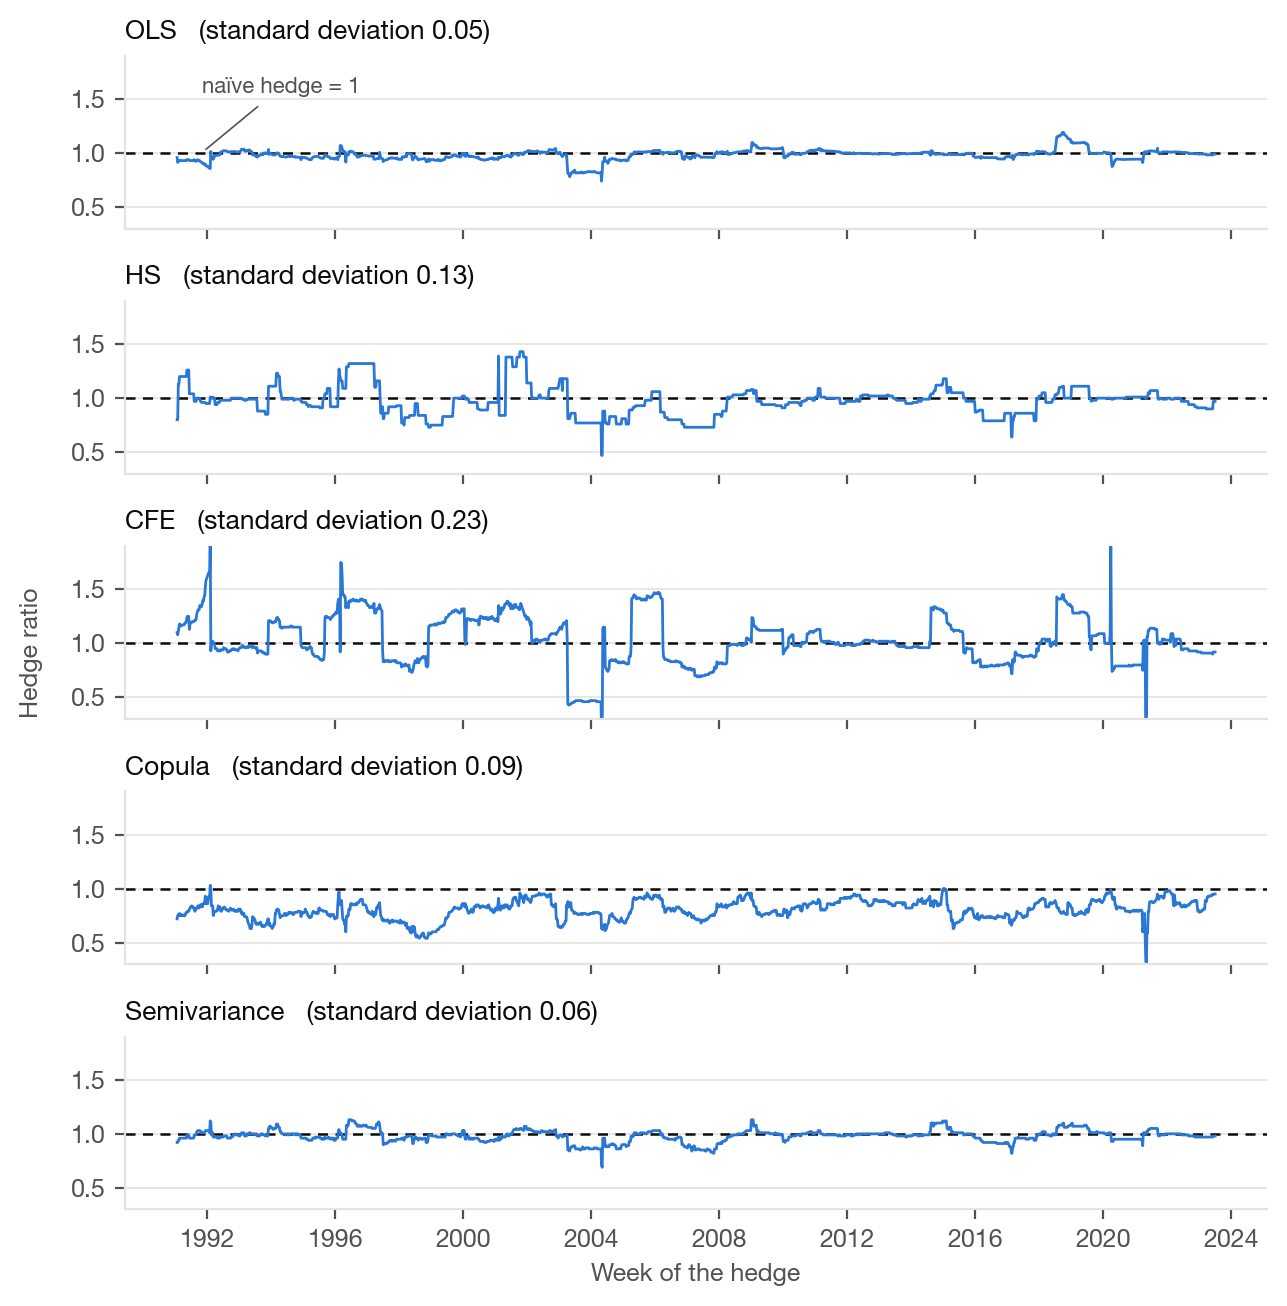
\includegraphics[width=5.0in]{../results/figures/fig1_hedge_ratios_wti.png}
\caption{Hedge ratios that minimize 5\% CVaR (downside), WTI, 52-week rolling window, 1991 to June 2023. The dashed line is the naïve ratio of one.}
\end{figure}

\begin{table}[!htb]
\caption{Hedge ratios that minimize 5\% CVaR (downside): mean and standard deviation over time}
\centering
\fontsize{9}{11.2}\selectfont\setlength{\tabcolsep}{3pt}
\begin{tabular}{@{}>{\raggedright\arraybackslash}p{\dimexpr 0.2031\linewidth-2\tabcolsep\relax}>{\centering\arraybackslash}p{\dimexpr 0.1594\linewidth-2\tabcolsep\relax}>{\centering\arraybackslash}p{\dimexpr 0.1594\linewidth-2\tabcolsep\relax}>{\centering\arraybackslash}p{\dimexpr 0.1594\linewidth-2\tabcolsep\relax}>{\centering\arraybackslash}p{\dimexpr 0.1594\linewidth-2\tabcolsep\relax}>{\centering\arraybackslash}p{\dimexpr 0.1594\linewidth-2\tabcolsep\relax}@{}}
\toprule
\textbf{Market} & \textbf{OLS} & \textbf{HS} & \textbf{CFE} & \textbf{Copula} & \textbf{Semivariance} \\
\midrule
WTI & 0.98 (0.05) & 0.97 (0.13) & 1.03 (0.23) & 0.81 (0.09) & 0.98 (0.06) \\
GBP/USD & 0.98 (0.03) & 1.00 (0.06) & 0.99 (0.07) & 0.80 (0.09) & 0.99 (0.03) \\
S\&P 500 & 0.98 (0.03) & 0.95 (0.08) & 0.97 (0.08) & 0.83 (0.08) & 0.96 (0.04) \\
Gold & 0.94 (0.05) & 0.92 (0.11) & 0.93 (0.13) & 0.72 (0.11) & 0.93 (0.06) \\
Bitcoin & 0.93 (0.05) & 0.95 (0.17) & 0.96 (0.16) & 0.64 (0.12) & 0.93 (0.10) \\
Natural gas & 1.00 (0.43) & 0.97 (0.31) & 1.03 (0.48) & 0.75 (0.22) & 0.99 (0.29) \\
\bottomrule
\end{tabular}
\par\vspace{3pt}\begin{minipage}{\linewidth}\footnotesize\raggedright \textit{Note.} Standard deviations in parentheses. Original sample for the first four markets (paper setting); full sample for Bitcoin and natural gas (same-contract setting). The naïve ratio is 1 with no variation. Ratios are limited to the range 0 to 2; the CFE ratio is at a limit in 12\% of natural gas weeks and almost never elsewhere (Appendix B).\end{minipage}
\end{table}

Table 8 is our addition to the paper's evidence. It puts numbers on the two sides of inequality (2). In every market the variance-minimizing ratio is close to one, between 0.95 and 1.00, so the bias of the naïve hedge is small. For OLS the noise is of the same order as that bias: it is 1.0 to 2.4 times the bias in WTI, GBP/USD, the S\&P 500 and gold, and slightly below it in Bitcoin. This is what the near-ties between the naïve and OLS hedges in Table 5 look like from the side of the hedge ratio: neither has a clear edge. For the tail-risk models the noise is far larger. The variance of the HS ratio is 5 to 22 times the naïve hedge's bias in the five markets other than natural gas, and the Cornish–Fisher ratio is noisier than the HS ratio in 4 of the six markets. Natural gas is the extreme case. Its variance-minimizing ratio is 0.999, so the naïve hedge has almost no bias, while its low $R^2$ of 0.32 makes every estimate noisy: there even the OLS ratio is noisier than the HS ratio. That is consistent with the OLS hedge being less effective than the naïve hedge in all 12 natural gas scenarios (Section 5.3).

Two cautions apply to Table 8. First, the noise columns contain two things: sampling error, and movement of the best ratio itself, which an estimate from the past year also fails to track. For OLS the two can be separated. Sampling error alone (equation 21 in Appendix C.5) gives 0.17 for WTI and 4.0 for natural gas, against 0.25 and 18.5 in the table. Most of the natural gas figure is therefore movement in the ratio, not sampling error, although either number is far above the naïve hedge's bias there. Second, the comparison is exact only for variance; for tail risk it is an indication, not a test. In variance terms the two hedges can be compared directly: out of sample the naïve hedge removes at least as much variance as the OLS hedge in 5 of the six markets, and in the sixth, the S\&P 500, the two differ only in the fifth decimal place (Table 24 in Appendix A). The match with Table 8 is broad, not exact market by market: in Bitcoin, where OLS noise is slightly below the bias, the naïve hedge is still ahead, and in the S\&P 500, where noise is twice the bias, the two tie. One reason is that the bias column uses a single whole-sample ratio, while the best ratio moves over time.

\begin{table}[!htb]
\caption{The cost of fixing the ratio at one against the noise of estimating it}
\centering
\fontsize{9}{11.2}\selectfont\setlength{\tabcolsep}{3pt}
\begin{tabular}{@{}>{\raggedright\arraybackslash}p{\dimexpr 0.1857\linewidth-2\tabcolsep\relax}>{\centering\arraybackslash}p{\dimexpr 0.1143\linewidth-2\tabcolsep\relax}>{\centering\arraybackslash}p{\dimexpr 0.1143\linewidth-2\tabcolsep\relax}>{\centering\arraybackslash}p{\dimexpr 0.1571\linewidth-2\tabcolsep\relax}>{\centering\arraybackslash}p{\dimexpr 0.1429\linewidth-2\tabcolsep\relax}>{\centering\arraybackslash}p{\dimexpr 0.1429\linewidth-2\tabcolsep\relax}>{\centering\arraybackslash}p{\dimexpr 0.1429\linewidth-2\tabcolsep\relax}@{}}
\toprule
\textbf{Market} & \textbf{$\beta$} & \textbf{$R^2$} & \textbf{Bias of naïve} & \textbf{Noise: OLS} & \textbf{Noise: HS} & \textbf{Noise: CFE} \\
\midrule
WTI & 0.968 & 0.92 & 0.103 & 0.245 & 1.803 & 5.116 \\
GBP/USD & 0.974 & 0.97 & 0.070 & 0.072 & 0.340 & 0.429 \\
S\&P 500 & 0.982 & 0.99 & 0.032 & 0.064 & 0.707 & 0.645 \\
Gold & 0.954 & 0.93 & 0.214 & 0.258 & 1.118 & 1.709 \\
Bitcoin & 0.947 & 0.89 & 0.276 & 0.234 & 2.747 & 2.629 \\
Natural gas & 0.999 & 0.32 & 0.000 & 18.471 & 9.418 & 22.879 \\
\bottomrule
\end{tabular}
\par\vspace{3pt}\begin{minipage}{\linewidth}\footnotesize\raggedright \textit{Note.} $\beta$ is the variance-minimizing hedge ratio and $R^2$ the share of spot variance explained by futures, both over the whole sample, including the first 52 weeks that the out-of-sample tables leave out. The bias of the naïve hedge is $(1-\beta)^2$. Noise is the variance over time of each model's ratio; for HS and CFE it is the 5\% CVaR (downside) ratio of Table 7. The last four columns are multiplied by 100 and correspond to the two sides of inequality (2). Variance over time includes genuine changes in the best ratio as well as sampling noise, so the noise columns are upper bounds on sampling noise. Samples as in Table 7.\end{minipage}
\end{table}

Second, the estimated models win in-sample, as they do in the paper's Table 9 (Table 22 in Appendix A gives our counts by model). Figure 2 counts the scenarios in which the naïve hedge is the best model when each ratio is evaluated on the weeks it was estimated on, and when it is applied to the following week. In-sample the naïve hedge is best in 1, 1, 0 and 0 of 12 scenarios in the four original markets and in 1 and 1 for Bitcoin and natural gas; the paper reports 1, 3, 3 and 3. Most of the models are therefore not badly specified: they do find ratios that would have reduced tail risk further (Section 6 takes them one by one). Third, that advantage does not survive the step to the next week: out-of-sample, the best estimated model loses on average 0.011 of effectiveness in the original markets relative to its in-sample result, which is the whole of its in-sample lead over the naïve hedge (0.011). In natural gas it loses 0.051, more than its in-sample lead of 0.034.

Unstable ratios, in-sample wins that do not carry over, and noise that exceeds the naïve hedge's bias are what estimation error predicts. Each prediction could have failed, in any of the six markets. One did, narrowly: in Bitcoin the OLS ratio's noise is slightly below the naïve hedge's bias (Table 8). The others held everywhere. That is the sense in which the evidence supports estimation error as the explanation (Section 6 gives its limits).

\begin{figure}[!htb]
\centering
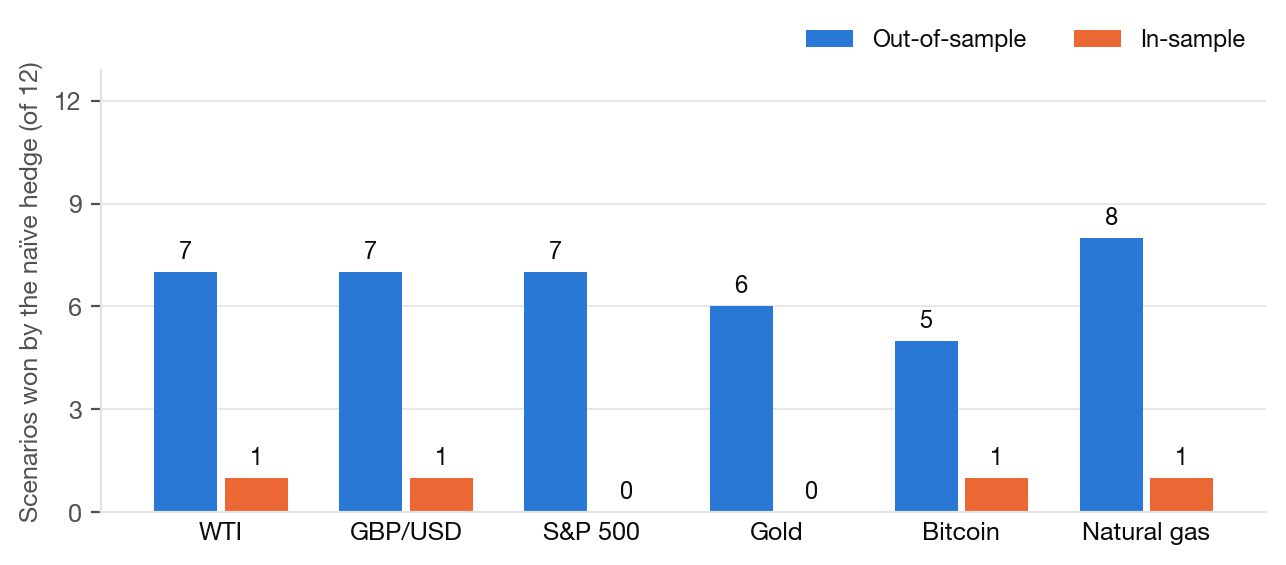
\includegraphics[width=5.2in]{../results/figures/fig2_naive_wins_in_vs_out.png}
\caption{Scenarios (of 12) in which the naïve hedge has the highest tail-risk effectiveness, out-of-sample and in-sample.}
\end{figure}

\subsection*{5.5 Basis risk and the economic cycle}

Table 9 repeats the paper's two conditional analyses, by basis risk (its Table 13) and by economic growth (its Tables 7 and 8), and uses the first to test the counterargument. If basis risk favored estimated ratios, the naïve hedge should win less often when the basis is volatile. Gold behaves this way: the naïve hedge wins 10 of 12 scenarios in calm-basis weeks and 0 in volatile-basis weeks, where OLS and the semivariance hedge are ahead, by at most 0.025 in effectiveness. This is the pattern in the paper's Table 13. It does not generalize. For the S\&P 500, Bitcoin and natural gas the naïve hedge wins more often when the basis is volatile (8, 8 and 8 of 12) than when it is calm (4, 3 and 4), and in volatile-basis weeks for natural gas the OLS hedge removes 13\% of the 5\% CVaR against 21\% for the naïve hedge. These are counts of wins, which Section 5.1 showed to be fragile, so the effectiveness columns of Table 9 carry more weight than the counts. On that measure the OLS hedge is ahead in volatile-basis weeks for gold and the S\&P 500, by 0.007 and 0.006, and behind for WTI, GBP/USD, Bitcoin and natural gas. Our reading is that a volatile basis has two effects. It makes the best ratio differ from one, which helps estimated models, and it makes that ratio harder to estimate from 52 weeks, which hurts them. For the variance-minimizing ratio the second effect has an exact form: the sampling variance of the OLS slope is proportional to $(1-R^2)/R^2$, which rises steeply as the link between spot and futures loosens (Appendix C.5). In natural gas the second effect clearly dominates; in Bitcoin, where the naïve hedge wins fewer scenarios overall, the evidence is weaker. We do not test this reading directly for the tail-risk models; doing so would need hedge ratios estimated on windows of different lengths.

\begin{table}[!htb]
\caption{Naïve and OLS hedges by basis volatility and by economic growth}
\centering
\fontsize{9}{11.2}\selectfont\setlength{\tabcolsep}{3pt}
\begin{tabular}{@{}>{\raggedright\arraybackslash}p{\dimexpr 0.2000\linewidth-2\tabcolsep\relax}>{\centering\arraybackslash}p{\dimexpr 0.2000\linewidth-2\tabcolsep\relax}>{\centering\arraybackslash}p{\dimexpr 0.2000\linewidth-2\tabcolsep\relax}>{\centering\arraybackslash}p{\dimexpr 0.2000\linewidth-2\tabcolsep\relax}>{\centering\arraybackslash}p{\dimexpr 0.2000\linewidth-2\tabcolsep\relax}@{}}
\toprule
\textbf{Market} & \textbf{Naïve wins (of 12)} & \textbf{OLS wins (of 12)} & \textbf{5\% CVaR HE, naïve} & \textbf{5\% CVaR HE, OLS} \\
\midrule
\multicolumn{5}{@{}l}{\textbf{\textit{By basis volatility: below median / above median}}} \\
WTI & 7 / 7 & 2 / 4 & 0.779 / 0.661 & 0.780 / 0.650 \\
GBP/USD & 4 / 6 & 4 / 5 & 0.857 / 0.881 & 0.858 / 0.867 \\
S\&P 500 & 4 / 8 & 5 / 3 & 0.911 / 0.835 & 0.909 / 0.841 \\
Gold & 10 / 0 & 2 / 6 & 0.792 / 0.681 & 0.792 / 0.687 \\
Bitcoin & 3 / 8 & 5 / 0 & 0.642 / 0.675 & 0.648 / 0.666 \\
Natural gas & 4 / 8 & 3 / 0 & 0.287 / 0.210 & 0.300 / 0.127 \\
\addlinespace[3pt]\multicolumn{5}{@{}l}{\textbf{\textit{By economic growth (CFNAI): below average / above average}}} \\
WTI & 6 / 7 & 5 / 4 & 0.717 / 0.697 & 0.705 / 0.701 \\
GBP/USD & 6 / 5 & 4 / 2 & 0.869 / 0.876 & 0.858 / 0.868 \\
S\&P 500 & 7 / 3 & 3 / 5 & 0.886 / 0.837 & 0.884 / 0.845 \\
Gold & 5 / 2 & 5 / 6 & 0.727 / 0.731 & 0.732 / 0.733 \\
Bitcoin & 7 / 3 & 0 / 6 & 0.686 / 0.620 & 0.680 / 0.621 \\
Natural gas & 10 / 9 & 0 / 0 & 0.229 / 0.242 & 0.156 / 0.167 \\
\bottomrule
\end{tabular}
\par\vspace{3pt}\begin{minipage}{\linewidth}\footnotesize\raggedright \textit{Note.} Out-of-sample. Basis volatility is the standard deviation of the weekly difference between spot and futures returns over the previous 52 weeks, split at its median. Original sample for the first four markets; full sample for Bitcoin and natural gas.\end{minipage}
\end{table}

The split by economic growth gives a weaker pattern than the paper reports. The naïve hedge wins more scenarios in weeks of below-average growth for the S\&P 500 (7 against 3), gold (5 against 2) and Bitcoin (7 against 3). For WTI, GBP/USD and natural gas the counts in the two regimes are within one of each other. In no market does the naïve hedge do clearly worse when growth is weak, which is when tail protection is most needed.

\subsection*{5.6 Stress episodes}

\begin{table}[!htb]
\caption{Worst weekly return of a long spot position in stress episodes: unhedged and hedged}
\centering
\fontsize{8.5}{10.6}\selectfont\setlength{\tabcolsep}{3pt}
\begin{tabular}{@{}>{\raggedright\arraybackslash}p{\dimexpr 0.2538\linewidth-2\tabcolsep\relax}>{\centering\arraybackslash}p{\dimexpr 0.1231\linewidth-2\tabcolsep\relax}>{\centering\arraybackslash}p{\dimexpr 0.0692\linewidth-2\tabcolsep\relax}>{\centering\arraybackslash}p{\dimexpr 0.1077\linewidth-2\tabcolsep\relax}>{\centering\arraybackslash}p{\dimexpr 0.1154\linewidth-2\tabcolsep\relax}>{\centering\arraybackslash}p{\dimexpr 0.2077\linewidth-2\tabcolsep\relax}>{\centering\arraybackslash}p{\dimexpr 0.1231\linewidth-2\tabcolsep\relax}@{}}
\toprule
\textbf{Episode} & \textbf{Market} & \textbf{Weeks} & \textbf{Unhedged} & \textbf{Naïve hedge} & \textbf{Best estimated model} & \textbf{Worst estimated model} \\
\midrule
COVID crash, Feb–Apr 2020 & WTI & 11 & −38.2\% & −15.7\% & −15.6\% (Copula) & −29.9\% \\
COVID crash, Feb–Apr 2020 & S\&P 500 & 11 & −12.5\% & −0.6\% & −0.7\% (Semivariance) & −10.8\% \\
COVID crash, Feb–Apr 2020 & Bitcoin & 11 & −32.1\% & −4.9\% & −3.3\% (HS) & −17.1\% \\
Winter Storm Uri, Feb 2021 & Natural gas & 4 & −88.3\% & −87.3\% & −86.5\% (OLS) & −87.6\% \\
FTX collapse, Nov 2022 & Bitcoin & 5 & −14.5\% & −8.4\% & −7.5\% (Copula) & −9.1\% \\
Yen carry unwind, Aug 2024 & S\&P 500 & 3 & −5.8\% & 0.1\% & 0.0\% (CFE) & −1.4\% \\
Yen carry unwind, Aug 2024 & Bitcoin & 3 & −15.2\% & −1.8\% & −1.0\% (HS) & −5.2\% \\
Tariff sell-off, Apr 2025 & WTI & 4 & −13.2\% & −0.1\% & −0.1\% (OLS) & −1.8\% \\
Tariff sell-off, Apr 2025 & S\&P 500 & 4 & −3.8\% & 0.1\% & 0.0\% (CFE) & −0.4\% \\
Tariff sell-off, Apr 2025 & Natural gas & 4 & −15.3\% & −10.0\% & −4.4\% (CFE) & −10.9\% \\
\bottomrule
\end{tabular}
\par\vspace{3pt}\begin{minipage}{\linewidth}\footnotesize\raggedright \textit{Note.} Out-of-sample hedge ratios that minimize 5\% CVaR. Simple weekly returns; a negative value is a loss. The best estimated model is known only after the fact. The table shows 10 of the 21 episode–market pairs we computed; all of them are in results/tables/stress\_events.csv in the repository.\end{minipage}
\end{table}

The paper does not examine individual episodes. Table 10 adds the ones named in our proposal, to look at the weeks that matter most. In the market-wide episodes the naïve hedge removes nearly all of the loss in the S\&P 500 and most of it in WTI and Bitcoin. The best estimated model, which can be identified only afterwards, is more than two percentage points ahead in 1 of the 21 episode–market pairs we computed, natural gas in April 2025. The column for the worst estimated model shows the other side of estimation. After the first weeks of the COVID crash the Cornish–Fisher ratio for WTI and the S\&P 500 jumped to 2, the upper limit of our search grid, and the over-hedged position then lost heavily when prices rebounded. Two episodes show the limits of any futures hedge. In Winter Storm Uri the loss came from a spot price that the futures did not follow, and in the FTX collapse the naïve hedge removed less than half of the worst weekly loss in Bitcoin's reference rate. The same is true of four pairs not shown in the table: gold in August 2024 and April 2025, and natural gas in March 2020 and August 2024. These are failures of the instrument, not of the hedge ratio: no estimated model did materially better.

\subsection*{5.7 Cost of the naïve hedge}

\begin{table}[!htb]
\caption{Opportunity cost of the naïve hedge: utility of the naïve hedge minus utility of each estimated model}
\centering
\fontsize{9}{11.2}\selectfont\setlength{\tabcolsep}{3pt}
\begin{tabular}{@{}>{\raggedright\arraybackslash}p{\dimexpr 0.1846\linewidth-2\tabcolsep\relax}>{\centering\arraybackslash}p{\dimexpr 0.1231\linewidth-2\tabcolsep\relax}>{\centering\arraybackslash}p{\dimexpr 0.1231\linewidth-2\tabcolsep\relax}>{\centering\arraybackslash}p{\dimexpr 0.1231\linewidth-2\tabcolsep\relax}>{\centering\arraybackslash}p{\dimexpr 0.1231\linewidth-2\tabcolsep\relax}>{\centering\arraybackslash}p{\dimexpr 0.1615\linewidth-2\tabcolsep\relax}>{\centering\arraybackslash}p{\dimexpr 0.1615\linewidth-2\tabcolsep\relax}@{}}
\toprule
\textbf{Market} & \textbf{OLS} & \textbf{HS} & \textbf{CFE} & \textbf{Copula} & \textbf{Semivariance} & \textbf{Smallest of 60} \\
\midrule
WTI & 0.0022 & 0.0047 & 0.0076 & 0.0099 & 0.0026 & 0.0022 \\
GBP/USD & 0.0015 & 0.0026 & 0.0034 & 0.0076 & 0.0017 & 0.0015 \\
S\&P 500 & 0.0012 & 0.0019 & 0.0028 & 0.0059 & 0.0015 & 0.0011 \\
Gold & 0.0027 & 0.0047 & 0.0053 & 0.0105 & 0.0030 & 0.0027 \\
Bitcoin & 0.0005 & 0.0013 & 0.0016 & 0.0054 & 0.0008 & 0.0005 \\
Natural gas & 0.0135 & 0.0142 & 0.0183 & 0.0248 & 0.0117 & 0.0093 \\
\bottomrule
\end{tabular}
\par\vspace{3pt}\begin{minipage}{\linewidth}\footnotesize\raggedright \textit{Note.} Mean–variance utility of weekly hedged returns with risk aversion 6, less transaction costs of 0.03\% of total turnover in the hedge ratio, as in the paper's equation 16. Average over the 12 scenarios. A positive value means the naïve hedge gives higher utility.\end{minipage}
\end{table}

A fixed ratio could still be costly if it gave up return or added variance in ordinary weeks. Table 11 follows the paper's calculation (its Table 11) and reaches the paper's result: the utility of the naïve hedge is higher than that of every estimated model in all six markets and in every one of the 360 scenario comparisons, and for WTI our OLS figure of 0.002 equals the paper's 0.002. The result should be read with care, because it comes almost entirely from trading costs. The formula sets the cost of all turnover over the sample against a weekly mean and variance, which gives costs a large weight. Before costs, the difference between the naïve and OLS hedges is between −0.0004 and 0.0000 in five of the six markets, too small to matter in either direction. Natural gas is the exception: there the naïve hedge is ahead of every estimated model before costs as well, by 0.002 to 0.004. The defensible conclusion is that the naïve hedge costs nothing in utility terms, not that it adds much.

\subsection*{5.8 Robustness}

\textit{Data conventions.} Re-running the original sample with same-contract returns and the flexible calendar gives 9, 10, 5 and 7 wins for the naïve hedge and, again, no significant test in favor of an estimated model. The conclusion does not depend on how roll weeks are treated. The level of effectiveness can. Applied to the weeks after June 2023, the paper's spliced returns put the naïve hedge's 5\% CVaR effectiveness for the S\&P 500 at 0.75, against 1.00 with same-contract returns. With interest rates above 4\%, each quarterly roll adds about 1.0\% to the spliced futures series, and these roll weeks become the short hedger's largest recorded “losses” although no hedger bears them. Studies that splice futures prices will understate hedging effectiveness whenever the futures curve is steep.

\textit{Natural gas spot source.} Using FRED alone, which restricts the evaluation to April 2008 onward (970 weeks), the naïve hedge wins 8 of 12 scenarios and no test favors an estimated model. \textit{Winter Storm Uri.} The two weeks of February 2021 in which the spot price spiked and fell back are by far the largest natural gas returns in the sample. Without them the naïve hedge still wins 8 of 12 scenarios, the OLS hedge is still less effective in 12 of 12 and no test favors an estimated model, while the share of variance removed by the naïve hedge rises from 32\% to 43\%. The natural gas result does not rest on that episode. \textit{Bitcoin spot source.} The CME reference rate is fixed in the London afternoon, several hours before the futures settle. With Bloomberg's closing Bitcoin price the naïve hedge's effectiveness rises to between 0.81 and 0.88, and it wins 6 of 12 scenarios with no significant test against it. The ranking is the same; the level depends on timing, as it does for GBP/USD and gold.

\textit{AI-concentration weeks.} Our proposal listed this as an optional check. It raised the possibility that the S\&P 500's recent tail risk, which is driven by a small number of AI-linked stocks, might behave differently. As a brief check we flagged the worst 10\% of weeks (Bloomberg total-return data) for the iShares Semiconductor ETF between July 2023 and November 2026 (18 weeks, with an average S\&P 500 return of −2.2\%). They include the week of the DeepSeek sell-off of January 27, 2025. In those weeks the naïve hedge removed 99.9\% of the squared S\&P 500 return, against 99.7\% in other weeks, and no estimated model differed from it by more than 0.1 percentage points. Index concentration changes what drives the S\&P 500, but not how closely its futures track it.

\section*{6. Discussion and Limitations}

Three alternative readings of the evidence deserve attention. The first is that the tests simply lack power, so that “not significantly better” means little. The paper's test does lack power here, because it treats two highly correlated series as independent. The paired test removes that weakness, and it moves the evidence toward the naïve hedge, not away from it. The second is that the estimated models are poor models. The in-sample results argue against this for three of the five. Evaluated on the weeks they were fitted to, the semivariance, HS and OLS hedges are more effective than the naïve hedge in 58, 52 and 47 of the 72 market–scenario pairs. The Cornish–Fisher hedge is ahead in only 30, so its out-of-sample losses may owe something to the approximation as well as to noise. The copula hedge is ahead in 7: it under-hedges by construction, in-sample and out-of-sample, and its failure is one of specification. The third is that a 52-week window is too short. We cannot rule this out. Our evidence is for a 52-week window only. We left the comparison of window lengths out when we narrowed the project in response to the feedback on our initial proposal, and the paper, whose method section mentions a 260-week window, reports results for 52 weeks only. A longer window would reduce noise in the estimates but would also respond more slowly to a change in the spot–futures relation, so the direction of the effect is not obvious. It is the first extension we would make, and it is also the direct test of our explanation: if estimation error is the cause, longer windows should reduce the noise in Table 8 and narrow the naïve hedge's lead. Our claim is therefore limited to this: with one year of weekly data, the results match what estimation error predicts in every respect we examined.

The results should be read with six limitations in mind. Our spot series for GBP/USD and gold are not the paper's, so hedging-effectiveness levels for those markets are not comparable with the published ones. The post-2023 sample and the Bitcoin sample are short, and conclusions at the 1\% level rest on two to four observations. Hedging effectiveness for natural gas and Bitcoin depends on which spot price is hedged; a firm exposed to a monthly index price would see a different basis from one exposed to Henry Hub daily spot. Our significance tests resample weeks independently, which ignores the clustering of volatile weeks and probably makes the counts of significant paired tests somewhat too large. We follow the paper's six models and do not consider dynamic hedge ratios, such as those from GARCH models. Finally, we study futures only. Options and other non-linear hedges address tail risk directly and are outside the scope of this project.

\section*{7. Conclusion}

This report asked whether the naïve hedge is still hard to beat for tail risk. It is. Rebuilding Cao and Conlon's (2025) study from raw data, we reach their central result for 1990 to June 2023: in each of the four markets the naïve hedge is the most effective model in at least as many scenarios as any estimated model, and the paper's test never favors an estimated model. The levels of effectiveness match the paper's for WTI and the S\&P 500; for GBP/USD and gold ours are higher, because our spot prices come from a different source.

Three more years of data and two new markets do not change the test result. From July 2023 to November 2026, and in Bitcoin and natural gas, the paper's test again never favors an estimated model. The scenario counts are less uniform. In the S\&P 500, where every model removes nearly all of the risk, the OLS hedge wins more scenarios than the naïve hedge once the new weeks are included, and in the weeks after June 2023 the paired test finds the OLS and Cornish–Fisher hedges significantly better in the 10\% downside scenarios, in every case by less than 0.01 in effectiveness. Both hypotheses are supported as we stated them: no estimated model significantly and consistently outperforms the naïve hedge. The significance tests are on VaR-type quantiles; CVaR and semivariance are compared by effectiveness only. Our paired test takes the result one step further than the paper. In 134 of the 192 distinct original-sample comparisons (86 of 144 without the copula model) the naïve hedge is not merely as good as the estimated model but significantly better, most often against the historical-simulation, Cornish–Fisher and copula models.

The pattern of results is the one that estimation error predicts. A hedge ratio fitted to the tail of one year of weekly data rests on a handful of observations. It moves sharply from week to week, it works on the weeks it was fitted to and not on the weeks that follow, and it costs more to trade. The naïve ratio has none of these problems because it is not estimated. Put as a trade-off between bias and variance, the naïve hedge accepts a small, fixed error, because the best ratio is close to one in every market we study, in exchange for removing an estimation error that is, for the tail-risk models, many times larger. One check did not fit: in Bitcoin the OLS ratio is slightly less noisy than the naïve hedge is biased. These findings are for a 52-week estimation window.

Basis risk, the main counterargument, does not rescue the estimated models. A volatile basis favors them in gold, but in natural gas, where spot and futures prices are least closely linked, the naïve hedge has its clearest lead. Two cautions apply. That lead is relative: futures remove only 32\% of the variance of natural gas spot returns, so every hedge there is weak and the naïve hedge is the best of them. And the Bitcoin evidence is thinner: the naïve hedge wins 5 of 12 scenarios in a sample of 411 weeks, although it is the market where a fixed ratio of one is furthest from the best ratio.

The replication also produced a point of method. The paper's futures returns appear to be spliced across contracts, which counts the price gap at each roll as a return. When the futures curve is steep this makes a hedge look worse than it is: after June 2023 it lowers the measured 5\% CVaR effectiveness of the naïve hedge for the S\&P 500 from 1.00 to 0.75 (Section 5.8). Studies of hedging effectiveness should compute each futures return on a single contract.

For a risk manager the lesson is that a hedge-ratio model is only as good as its inputs. For weekly tail risk estimated on a one-year window those inputs are too noisy to help. Where a liquid futures contract exists on the asset being hedged, the one-for-one hedge is the sensible default, and the case for replacing it has to be made out of sample and net of trading costs. Effort is better spent on the basis itself: choosing the contract, matching the timing of the exposure, and recognizing, as in natural gas, when the instrument cannot remove the risk at any ratio.

\section*{Group Member Contributions}

Each member was responsible for a distinct part of the analysis and for the corresponding parts of this report and of the presentation, as set out in our revised proposal. The literature review, the discussion and the conclusion were written jointly. Methodology decisions were made together.

\textbf{Hina Tomar.} Bloomberg and FRED data for the six markets; the rolled futures series; the naïve, OLS and historical-simulation hedges; the extension of the sample to 2026 (H1). Wrote the data and core replication parts.

\textbf{Kavin Dhanasekaran.} The Cornish–Fisher, Clayton copula and semivariance hedges; hedge-ratio stability; the in-sample versus out-of-sample comparison (estimation error). Wrote the model and estimation-error parts.

\textbf{Sai Kishore.} The evaluation framework (hedging effectiveness, the Wilcox test and utility); the basis-risk and CFNAI analysis; Bitcoin and natural gas (H2) and the stress episodes. Wrote the evaluation and new-market parts.

\section*{Use of AI Tools}

We used Claude, an AI assistant made by Anthropic, throughout this project, through its coding tool Claude Code. It wrote and tested most of the Python code under our direction, helped audit the data, ran the analysis, and drafted and edited the text of this report. The team chose the paper, the hypotheses and the research design, made the methodology decisions, and reviewed the code, the results and the text. We take responsibility for all content, including any errors.

\section*{References}

{\small\setlength{\parskip}{0pt}\interlinepenalty=10000\hangindent=0.3in\hangafter=1\noindent Aquilina, M., Lombardi, M., Schrimpf, A., \& Sushko, V. (2024). \textit{The market turbulence and carry trade unwind of August 2024} (BIS Bulletin No. 90). Bank for International Settlements. \url{https://www.bis.org/publ/bisbull90.htm}\par}

{\small\setlength{\parskip}{0pt}\interlinepenalty=10000\hangindent=0.3in\hangafter=1\noindent Basel Committee on Banking Supervision. (2019). \textit{Minimum capital requirements for market risk}. Bank for International Settlements. \url{https://www.bis.org/bcbs/publ/d457.htm}\par}

{\small\setlength{\parskip}{0pt}\interlinepenalty=10000\hangindent=0.3in\hangafter=1\noindent Bloomberg L.P. (2026). \textit{Bloomberg Terminal} [Spot and futures price data]. Accessed through New York University.\par}

{\small\setlength{\parskip}{0pt}\interlinepenalty=10000\hangindent=0.3in\hangafter=1\noindent Cao, M., \& Conlon, T. (2025). Tail risk hedging: The superiority of the naïve hedging strategy. \textit{Journal of Futures Markets, 45}(8), 977–1005. \url{https://doi.org/10.1002/fut.22602}\par}

{\small\setlength{\parskip}{0pt}\interlinepenalty=10000\hangindent=0.3in\hangafter=1\noindent Cao, Z., Harris, R. D. F., \& Shen, J. (2010). Hedging and value at risk: A semi-parametric approach. \textit{Journal of Futures Markets, 30}(8), 780–794. \url{https://doi.org/10.1002/fut.20440}\par}

{\small\setlength{\parskip}{0pt}\interlinepenalty=10000\hangindent=0.3in\hangafter=1\noindent Clayton, D. G. (1978). A model for association in bivariate life tables and its application in epidemiological studies of familial tendency in chronic disease incidence. \textit{Biometrika, 65}(1), 141–151. \url{https://doi.org/10.1093/biomet/65.1.141}\par}

{\small\setlength{\parskip}{0pt}\interlinepenalty=10000\hangindent=0.3in\hangafter=1\noindent Conlon, T., \& Cotter, J. (2013). Downside risk and the energy hedger’s horizon. \textit{Energy Economics, 36}, 371–379. \url{https://doi.org/10.1016/j.eneco.2012.09.012}\par}

{\small\setlength{\parskip}{0pt}\interlinepenalty=10000\hangindent=0.3in\hangafter=1\noindent Cotter, J., \& Hanly, J. (2006). Reevaluating hedging performance. \textit{Journal of Futures Markets, 26}(7), 677–702. \url{https://doi.org/10.1002/fut.20212}\par}

{\small\setlength{\parskip}{0pt}\interlinepenalty=10000\hangindent=0.3in\hangafter=1\noindent DeMiguel, V., Garlappi, L., \& Uppal, R. (2009). Optimal versus naive diversification: How inefficient is the 1/N portfolio strategy? \textit{Review of Financial Studies, 22}(5), 1915–1953. \url{https://doi.org/10.1093/rfs/hhm075}\par}

{\small\setlength{\parskip}{0pt}\interlinepenalty=10000\hangindent=0.3in\hangafter=1\noindent Ederington, L. H. (1979). The hedging performance of the new futures markets. \textit{Journal of Finance, 34}(1), 157–170. \url{https://doi.org/10.1111/j.1540-6261.1979.tb02077.x}\par}

{\small\setlength{\parskip}{0pt}\interlinepenalty=10000\hangindent=0.3in\hangafter=1\noindent Federal Energy Regulatory Commission (FERC) \& North American Electric Reliability Corporation (NERC). (2021). \textit{The February 2021 cold weather outages in Texas and the South Central United States} [Staff report]. \url{https://www.ferc.gov/media/february-2021-cold-weather-outages-texas-and-south-central-united-states-ferc-nerc-and}\par}

{\small\setlength{\parskip}{0pt}\interlinepenalty=10000\hangindent=0.3in\hangafter=1\noindent Federal Reserve Bank of St. Louis. (2026). \textit{Federal Reserve Economic Data (FRED)}: series CFNAI, DHHNGSP and DCOILWTICO [Data sets]. \url{https://fred.stlouisfed.org}\par}

{\small\setlength{\parskip}{0pt}\interlinepenalty=10000\hangindent=0.3in\hangafter=1\noindent Gensler, G. (2024, January 10). \textit{Statement on the approval of spot bitcoin exchange-traded products}. U.S. Securities and Exchange Commission. \url{https://www.sec.gov/newsroom/speeches-statements/gensler-statement-spot-bitcoin-011023}\par}

{\small\setlength{\parskip}{0pt}\interlinepenalty=10000\hangindent=0.3in\hangafter=1\noindent Harrell, F. E., \& Davis, C. E. (1982). A new distribution-free quantile estimator. \textit{Biometrika, 69}(3), 635–640. \url{https://doi.org/10.1093/biomet/69.3.635}\par}

{\small\setlength{\parskip}{0pt}\interlinepenalty=10000\hangindent=0.3in\hangafter=1\noindent Harris, R. D. F., \& Shen, J. (2006). Hedging and value at risk. \textit{Journal of Futures Markets, 26}(4), 369–390. \url{https://doi.org/10.1002/fut.20195}\par}

{\small\setlength{\parskip}{0pt}\interlinepenalty=10000\hangindent=0.3in\hangafter=1\noindent International Monetary Fund. (2025). \textit{Global financial stability report: Enhancing resilience amid uncertainty} (April 2025). \url{https://www.imf.org/en/Publications/GFSR/Issues/2025/04/22/global-financial-stability-report-april-2025}\par}

{\small\setlength{\parskip}{0pt}\interlinepenalty=10000\hangindent=0.3in\hangafter=1\noindent Wang, Y., Wu, C., \& Yang, L. (2015). Hedging with futures: Does anything beat the naïve hedging strategy? \textit{Management Science, 61}(12), 2870–2889. \url{https://doi.org/10.1287/mnsc.2014.2028}\par}

{\small\setlength{\parskip}{0pt}\interlinepenalty=10000\hangindent=0.3in\hangafter=1\noindent Wilcox, R. R., Erceg-Hurn, D. M., Clark, F., \& Carlson, M. (2014). Comparing two independent groups via the lower and upper quantiles. \textit{Journal of Statistical Computation and Simulation, 84}(7), 1543–1551. \url{https://doi.org/10.1080/00949655.2012.754026}\par}

\clearpage

\section*{Appendix A. Full Out-of-Sample Results}

{\small Each table reports tail-risk hedging effectiveness for the 12 scenarios, with the p-value of the Wilcox et al. (2014) test against the naïve hedge in parentheses. The best model in each column is in bold. Columns 1–6 are downside risk and columns 7–12 upside risk. Tables 12 to 17 are the main results: the replication for the four original markets and the full sample for Bitcoin and natural gas. Tables 18 to 21 give the four original markets over the whole period, January 1990 to November 2026, in the same-contract setting; Panel C of Table 5 summarizes them. All ten follow the layout of the paper's Table 5. Tables 22 to 24 supplement them: Table 22 is the counterpart of the paper's Table 9, Table 23 breaks down our paired test by model, and Table 24 is the counterpart of the paper's Table 6.\par}

\begin{table}[H]
\caption{WTI: hedging effectiveness and p-values, January 1990 to June 2023, paper setting (1,656 weeks)}
\centering
\fontsize{7.5}{9.4}\selectfont\setlength{\tabcolsep}{3pt}
\begin{tabular}{@{}>{\raggedright\arraybackslash}p{\dimexpr 0.1508\linewidth-2\tabcolsep\relax}>{\centering\arraybackslash}p{\dimexpr 0.0708\linewidth-2\tabcolsep\relax}>{\centering\arraybackslash}p{\dimexpr 0.0708\linewidth-2\tabcolsep\relax}>{\centering\arraybackslash}p{\dimexpr 0.0708\linewidth-2\tabcolsep\relax}>{\centering\arraybackslash}p{\dimexpr 0.0708\linewidth-2\tabcolsep\relax}>{\centering\arraybackslash}p{\dimexpr 0.0708\linewidth-2\tabcolsep\relax}>{\centering\arraybackslash}p{\dimexpr 0.0708\linewidth-2\tabcolsep\relax}>{\centering\arraybackslash}p{\dimexpr 0.0708\linewidth-2\tabcolsep\relax}>{\centering\arraybackslash}p{\dimexpr 0.0708\linewidth-2\tabcolsep\relax}>{\centering\arraybackslash}p{\dimexpr 0.0708\linewidth-2\tabcolsep\relax}>{\centering\arraybackslash}p{\dimexpr 0.0708\linewidth-2\tabcolsep\relax}>{\centering\arraybackslash}p{\dimexpr 0.0708\linewidth-2\tabcolsep\relax}>{\centering\arraybackslash}p{\dimexpr 0.0708\linewidth-2\tabcolsep\relax}@{}}
\toprule
 & \textbf{VaR 10\%} & \textbf{VaR 5\%} & \textbf{VaR 1\%} & \textbf{CVaR 10\%} & \textbf{CVaR 5\%} & \textbf{CVaR 1\%} & \textbf{VaR 90\%} & \textbf{VaR 95\%} & \textbf{VaR 99\%} & \textbf{CVaR 90\%} & \textbf{CVaR 95\%} & \textbf{CVaR 99\%} \\
\midrule
Naïve & 0.873 & 0.824 & \textbf{0.669} & \textbf{0.760} & \textbf{0.707} & \textbf{0.625} & \textbf{0.862} & \textbf{0.811} & 0.612 & \textbf{0.737} & 0.677 & 0.571 \\
OLS & 0.866 & \textbf{0.824} & 0.651 & 0.752 & 0.701 & 0.619 & 0.848 & 0.786 & \textbf{0.632} & 0.729 & \textbf{0.678} & \textbf{0.586} \\
 & (0.78) & (0.55) & (0.56) & (0.78) & (0.55) & (0.56) & (0.89) & (0.75) & (0.42) & (0.89) & (0.75) & (0.42) \\
HS & 0.865 & 0.780 & 0.599 & 0.751 & 0.683 & 0.562 & 0.853 & 0.778 & 0.590 & 0.730 & 0.647 & 0.453 \\
 & (0.80) & (0.94) & (0.68) & (0.88) & (0.98) & (0.95) & (0.84) & (0.90) & (0.61) & (0.98) & (0.99) & (0.97) \\
CFE & \textbf{0.877} & 0.822 & 0.567 & 0.703 & 0.618 & 0.502 & 0.859 & 0.796 & 0.493 & 0.652 & 0.552 & 0.352 \\
 & (0.43) & (0.65) & (0.82) & (1.00) & (1.00) & (0.93) & (0.62) & (0.66) & (0.90) & (1.00) & (1.00) & (0.96) \\
Copula & 0.834 & 0.774 & 0.605 & 0.712 & 0.659 & 0.571 & 0.819 & 0.722 & 0.432 & 0.661 & 0.577 & 0.411 \\
 & (1.00) & (0.98) & (0.80) & (1.00) & (1.00) & (0.87) & (1.00) & (1.00) & (0.99) & (1.00) & (1.00) & (1.00) \\
Semivariance & 0.869 & 0.823 & 0.667 & 0.752 & 0.701 & 0.621 & 0.831 & 0.780 & 0.607 & 0.710 & 0.654 & 0.541 \\
 & (0.75) & (0.57) & (0.53) & (0.75) & (0.57) & (0.53) & (0.99) & (0.85) & (0.60) & (0.99) & (0.85) & (0.60) \\
\bottomrule
\end{tabular}
\end{table}

\begin{table}[H]
\caption{GBP/USD: hedging effectiveness and p-values, January 1990 to June 2023, paper setting (1,675 weeks)}
\centering
\fontsize{7.5}{9.4}\selectfont\setlength{\tabcolsep}{3pt}
\begin{tabular}{@{}>{\raggedright\arraybackslash}p{\dimexpr 0.1508\linewidth-2\tabcolsep\relax}>{\centering\arraybackslash}p{\dimexpr 0.0708\linewidth-2\tabcolsep\relax}>{\centering\arraybackslash}p{\dimexpr 0.0708\linewidth-2\tabcolsep\relax}>{\centering\arraybackslash}p{\dimexpr 0.0708\linewidth-2\tabcolsep\relax}>{\centering\arraybackslash}p{\dimexpr 0.0708\linewidth-2\tabcolsep\relax}>{\centering\arraybackslash}p{\dimexpr 0.0708\linewidth-2\tabcolsep\relax}>{\centering\arraybackslash}p{\dimexpr 0.0708\linewidth-2\tabcolsep\relax}>{\centering\arraybackslash}p{\dimexpr 0.0708\linewidth-2\tabcolsep\relax}>{\centering\arraybackslash}p{\dimexpr 0.0708\linewidth-2\tabcolsep\relax}>{\centering\arraybackslash}p{\dimexpr 0.0708\linewidth-2\tabcolsep\relax}>{\centering\arraybackslash}p{\dimexpr 0.0708\linewidth-2\tabcolsep\relax}>{\centering\arraybackslash}p{\dimexpr 0.0708\linewidth-2\tabcolsep\relax}>{\centering\arraybackslash}p{\dimexpr 0.0708\linewidth-2\tabcolsep\relax}@{}}
\toprule
 & \textbf{VaR 10\%} & \textbf{VaR 5\%} & \textbf{VaR 1\%} & \textbf{CVaR 10\%} & \textbf{CVaR 5\%} & \textbf{CVaR 1\%} & \textbf{VaR 90\%} & \textbf{VaR 95\%} & \textbf{VaR 99\%} & \textbf{CVaR 90\%} & \textbf{CVaR 95\%} & \textbf{CVaR 99\%} \\
\midrule
Naïve & \textbf{0.871} & \textbf{0.865} & \textbf{0.869} & \textbf{0.871} & \textbf{0.873} & \textbf{0.887} & 0.862 & \textbf{0.842} & 0.768 & 0.809 & 0.784 & 0.731 \\
OLS & 0.867 & 0.860 & 0.855 & 0.864 & 0.864 & 0.878 & \textbf{0.867} & 0.828 & \textbf{0.768} & \textbf{0.810} & \textbf{0.787} & 0.746 \\
 & (0.73) & (0.72) & (0.78) & (0.73) & (0.72) & (0.78) & (0.42) & (0.67) & (0.50) & (0.42) & (0.67) & (0.50) \\
HS & 0.864 & 0.857 & 0.857 & 0.867 & 0.862 & 0.833 & 0.852 & 0.806 & 0.730 & 0.801 & 0.771 & 0.676 \\
 & (0.80) & (0.81) & (0.83) & (0.82) & (0.89) & (0.98) & (0.78) & (0.97) & (0.93) & (0.82) & (0.98) & (0.98) \\
CFE & 0.865 & 0.860 & 0.845 & 0.861 & 0.854 & 0.851 & 0.862 & 0.821 & 0.732 & 0.797 & 0.754 & 0.628 \\
 & (0.81) & (0.72) & (0.91) & (0.84) & (0.86) & (0.91) & (0.60) & (0.84) & (0.91) & (0.87) & (0.98) & (0.97) \\
Copula & 0.846 & 0.786 & 0.711 & 0.777 & 0.742 & 0.684 & 0.844 & 0.784 & 0.597 & 0.762 & 0.692 & 0.442 \\
 & (1.00) & (1.00) & (1.00) & (1.00) & (1.00) & (1.00) & (0.95) & (1.00) & (1.00) & (1.00) & (1.00) & (1.00) \\
Semivariance & 0.867 & 0.862 & 0.866 & 0.868 & 0.870 & 0.886 & 0.855 & 0.826 & 0.759 & 0.806 & 0.786 & \textbf{0.750} \\
 & (0.72) & (0.66) & (0.56) & (0.72) & (0.66) & (0.56) & (0.75) & (0.80) & (0.56) & (0.75) & (0.80) & (0.56) \\
\bottomrule
\end{tabular}
\end{table}

\begin{table}[H]
\caption{S\&P 500: hedging effectiveness and p-values, January 1990 to June 2023, paper setting (1,675 weeks)}
\centering
\fontsize{7.5}{9.4}\selectfont\setlength{\tabcolsep}{3pt}
\begin{tabular}{@{}>{\raggedright\arraybackslash}p{\dimexpr 0.1508\linewidth-2\tabcolsep\relax}>{\centering\arraybackslash}p{\dimexpr 0.0708\linewidth-2\tabcolsep\relax}>{\centering\arraybackslash}p{\dimexpr 0.0708\linewidth-2\tabcolsep\relax}>{\centering\arraybackslash}p{\dimexpr 0.0708\linewidth-2\tabcolsep\relax}>{\centering\arraybackslash}p{\dimexpr 0.0708\linewidth-2\tabcolsep\relax}>{\centering\arraybackslash}p{\dimexpr 0.0708\linewidth-2\tabcolsep\relax}>{\centering\arraybackslash}p{\dimexpr 0.0708\linewidth-2\tabcolsep\relax}>{\centering\arraybackslash}p{\dimexpr 0.0708\linewidth-2\tabcolsep\relax}>{\centering\arraybackslash}p{\dimexpr 0.0708\linewidth-2\tabcolsep\relax}>{\centering\arraybackslash}p{\dimexpr 0.0708\linewidth-2\tabcolsep\relax}>{\centering\arraybackslash}p{\dimexpr 0.0708\linewidth-2\tabcolsep\relax}>{\centering\arraybackslash}p{\dimexpr 0.0708\linewidth-2\tabcolsep\relax}>{\centering\arraybackslash}p{\dimexpr 0.0708\linewidth-2\tabcolsep\relax}@{}}
\toprule
 & \textbf{VaR 10\%} & \textbf{VaR 5\%} & \textbf{VaR 1\%} & \textbf{CVaR 10\%} & \textbf{CVaR 5\%} & \textbf{CVaR 1\%} & \textbf{VaR 90\%} & \textbf{VaR 95\%} & \textbf{VaR 99\%} & \textbf{CVaR 90\%} & \textbf{CVaR 95\%} & \textbf{CVaR 99\%} \\
\midrule
Naïve & \textbf{0.896} & \textbf{0.882} & 0.848 & 0.875 & 0.864 & 0.866 & \textbf{0.880} & 0.882 & \textbf{0.894} & \textbf{0.888} & \textbf{0.890} & \textbf{0.903} \\
OLS & 0.893 & 0.881 & \textbf{0.852} & \textbf{0.875} & \textbf{0.867} & \textbf{0.869} & 0.879 & \textbf{0.885} & 0.888 & 0.887 & 0.889 & 0.899 \\
 & (0.67) & (0.57) & (0.43) & (0.67) & (0.57) & (0.43) & (0.55) & (0.44) & (0.69) & (0.55) & (0.44) & (0.69) \\
HS & 0.896 & 0.868 & 0.820 & 0.871 & 0.853 & 0.844 & 0.876 & 0.880 & 0.888 & 0.885 & 0.886 & 0.883 \\
 & (0.65) & (0.92) & (0.95) & (0.86) & (0.95) & (0.96) & (0.68) & (0.63) & (0.86) & (0.47) & (0.72) & (0.97) \\
CFE & 0.888 & 0.872 & 0.815 & 0.866 & 0.828 & 0.746 & 0.880 & 0.884 & 0.880 & 0.883 & 0.852 & 0.772 \\
 & (0.82) & (0.84) & (0.95) & (0.91) & (0.90) & (0.99) & (0.45) & (0.38) & (0.94) & (0.57) & (0.48) & (0.97) \\
Copula & 0.879 & 0.832 & 0.796 & 0.833 & 0.812 & 0.795 & 0.872 & 0.841 & 0.676 & 0.838 & 0.786 & 0.649 \\
 & (0.99) & (1.00) & (1.00) & (1.00) & (1.00) & (1.00) & (0.91) & (1.00) & (1.00) & (1.00) & (1.00) & (1.00) \\
Semivariance & 0.889 & 0.876 & 0.852 & 0.872 & 0.864 & 0.868 & 0.879 & 0.882 & 0.889 & 0.886 & 0.888 & 0.896 \\
 & (0.81) & (0.72) & (0.45) & (0.81) & (0.72) & (0.45) & (0.49) & (0.57) & (0.75) & (0.49) & (0.57) & (0.75) \\
\bottomrule
\end{tabular}
\end{table}

\begin{table}[H]
\caption{Gold: hedging effectiveness and p-values, January 1990 to June 2023, paper setting (1,675 weeks)}
\centering
\fontsize{7.5}{9.4}\selectfont\setlength{\tabcolsep}{3pt}
\begin{tabular}{@{}>{\raggedright\arraybackslash}p{\dimexpr 0.1508\linewidth-2\tabcolsep\relax}>{\centering\arraybackslash}p{\dimexpr 0.0708\linewidth-2\tabcolsep\relax}>{\centering\arraybackslash}p{\dimexpr 0.0708\linewidth-2\tabcolsep\relax}>{\centering\arraybackslash}p{\dimexpr 0.0708\linewidth-2\tabcolsep\relax}>{\centering\arraybackslash}p{\dimexpr 0.0708\linewidth-2\tabcolsep\relax}>{\centering\arraybackslash}p{\dimexpr 0.0708\linewidth-2\tabcolsep\relax}>{\centering\arraybackslash}p{\dimexpr 0.0708\linewidth-2\tabcolsep\relax}>{\centering\arraybackslash}p{\dimexpr 0.0708\linewidth-2\tabcolsep\relax}>{\centering\arraybackslash}p{\dimexpr 0.0708\linewidth-2\tabcolsep\relax}>{\centering\arraybackslash}p{\dimexpr 0.0708\linewidth-2\tabcolsep\relax}>{\centering\arraybackslash}p{\dimexpr 0.0708\linewidth-2\tabcolsep\relax}>{\centering\arraybackslash}p{\dimexpr 0.0708\linewidth-2\tabcolsep\relax}>{\centering\arraybackslash}p{\dimexpr 0.0708\linewidth-2\tabcolsep\relax}@{}}
\toprule
 & \textbf{VaR 10\%} & \textbf{VaR 5\%} & \textbf{VaR 1\%} & \textbf{CVaR 10\%} & \textbf{CVaR 5\%} & \textbf{CVaR 1\%} & \textbf{VaR 90\%} & \textbf{VaR 95\%} & \textbf{VaR 99\%} & \textbf{CVaR 90\%} & \textbf{CVaR 95\%} & \textbf{CVaR 99\%} \\
\midrule
Naïve & \textbf{0.745} & \textbf{0.741} & 0.747 & 0.733 & 0.728 & 0.720 & \textbf{0.812} & 0.775 & \textbf{0.754} & \textbf{0.762} & \textbf{0.741} & 0.693 \\
OLS & 0.741 & 0.738 & \textbf{0.749} & \textbf{0.735} & \textbf{0.732} & \textbf{0.724} & 0.801 & \textbf{0.781} & 0.744 & 0.760 & 0.739 & \textbf{0.694} \\
 & (0.56) & (0.50) & (0.38) & (0.56) & (0.50) & (0.38) & (0.77) & (0.43) & (0.47) & (0.77) & (0.43) & (0.47) \\
HS & 0.722 & 0.720 & 0.679 & 0.726 & 0.703 & 0.621 & 0.802 & 0.774 & 0.698 & 0.757 & 0.714 & 0.634 \\
 & (0.90) & (0.89) & (0.97) & (0.72) & (0.82) & (1.00) & (0.76) & (0.63) & (0.89) & (0.80) & (0.71) & (0.93) \\
CFE & 0.738 & 0.738 & 0.662 & 0.711 & 0.676 & 0.572 & 0.804 & 0.779 & 0.691 & 0.749 & 0.713 & 0.605 \\
 & (0.60) & (0.60) & (1.00) & (0.85) & (0.98) & (1.00) & (0.71) & (0.38) & (0.91) & (0.95) & (0.86) & (0.99) \\
Copula & 0.710 & 0.675 & 0.638 & 0.660 & 0.620 & 0.569 & 0.790 & 0.741 & 0.436 & 0.716 & 0.643 & 0.337 \\
 & (0.98) & (1.00) & (1.00) & (1.00) & (1.00) & (1.00) & (0.91) & (0.98) & (1.00) & (1.00) & (1.00) & (1.00) \\
Semivariance & 0.733 & 0.739 & 0.741 & 0.726 & 0.722 & 0.716 & 0.802 & 0.780 & 0.725 & 0.758 & 0.737 & 0.693 \\
 & (0.75) & (0.59) & (0.61) & (0.75) & (0.59) & (0.61) & (0.78) & (0.51) & (0.61) & (0.78) & (0.51) & (0.61) \\
\bottomrule
\end{tabular}
\end{table}

\begin{table}[H]
\caption{Bitcoin: hedging effectiveness and p-values, full sample, same-contract setting (411 weeks)}
\centering
\fontsize{7.5}{9.4}\selectfont\setlength{\tabcolsep}{3pt}
\begin{tabular}{@{}>{\raggedright\arraybackslash}p{\dimexpr 0.1508\linewidth-2\tabcolsep\relax}>{\centering\arraybackslash}p{\dimexpr 0.0708\linewidth-2\tabcolsep\relax}>{\centering\arraybackslash}p{\dimexpr 0.0708\linewidth-2\tabcolsep\relax}>{\centering\arraybackslash}p{\dimexpr 0.0708\linewidth-2\tabcolsep\relax}>{\centering\arraybackslash}p{\dimexpr 0.0708\linewidth-2\tabcolsep\relax}>{\centering\arraybackslash}p{\dimexpr 0.0708\linewidth-2\tabcolsep\relax}>{\centering\arraybackslash}p{\dimexpr 0.0708\linewidth-2\tabcolsep\relax}>{\centering\arraybackslash}p{\dimexpr 0.0708\linewidth-2\tabcolsep\relax}>{\centering\arraybackslash}p{\dimexpr 0.0708\linewidth-2\tabcolsep\relax}>{\centering\arraybackslash}p{\dimexpr 0.0708\linewidth-2\tabcolsep\relax}>{\centering\arraybackslash}p{\dimexpr 0.0708\linewidth-2\tabcolsep\relax}>{\centering\arraybackslash}p{\dimexpr 0.0708\linewidth-2\tabcolsep\relax}>{\centering\arraybackslash}p{\dimexpr 0.0708\linewidth-2\tabcolsep\relax}@{}}
\toprule
 & \textbf{VaR 10\%} & \textbf{VaR 5\%} & \textbf{VaR 1\%} & \textbf{CVaR 10\%} & \textbf{CVaR 5\%} & \textbf{CVaR 1\%} & \textbf{VaR 90\%} & \textbf{VaR 95\%} & \textbf{VaR 99\%} & \textbf{CVaR 90\%} & \textbf{CVaR 95\%} & \textbf{CVaR 99\%} \\
\midrule
Naïve & 0.595 & 0.605 & \textbf{0.658} & \textbf{0.648} & \textbf{0.658} & \textbf{0.730} & 0.672 & \textbf{0.721} & 0.601 & 0.687 & 0.687 & 0.632 \\
OLS & 0.593 & \textbf{0.607} & 0.655 & 0.645 & 0.654 & 0.714 & 0.651 & 0.705 & 0.669 & 0.685 & 0.689 & 0.654 \\
 & (0.52) & (0.49) & (0.48) & (0.52) & (0.49) & (0.48) & (0.63) & (0.71) & (0.35) & (0.63) & (0.71) & (0.35) \\
HS & \textbf{0.599} & 0.590 & 0.554 & 0.627 & 0.613 & 0.630 & \textbf{0.673} & 0.690 & 0.680 & 0.682 & 0.690 & 0.655 \\
 & (0.50) & (0.69) & (0.89) & (0.64) & (0.82) & (0.91) & (0.62) & (0.90) & (0.24) & (0.75) & (0.90) & (0.44) \\
CFE & 0.581 & 0.595 & 0.560 & 0.604 & 0.592 & 0.651 & 0.642 & 0.694 & 0.682 & 0.677 & 0.681 & 0.622 \\
 & (0.59) & (0.70) & (0.93) & (0.76) & (0.75) & (0.96) & (0.70) & (0.81) & (0.24) & (0.78) & (0.90) & (0.49) \\
Copula & 0.527 & 0.556 & 0.568 & 0.516 & 0.487 & 0.432 & 0.647 & 0.664 & 0.390 & 0.620 & 0.552 & 0.345 \\
 & (0.88) & (0.94) & (0.95) & (0.97) & (0.96) & (0.96) & (0.76) & (0.99) & (1.00) & (0.90) & (1.00) & (1.00) \\
Semivariance & 0.561 & 0.591 & 0.624 & 0.623 & 0.639 & 0.700 & 0.658 & 0.701 & \textbf{0.686} & \textbf{0.687} & \textbf{0.699} & \textbf{0.686} \\
 & (0.72) & (0.68) & (0.64) & (0.72) & (0.68) & (0.64) & (0.69) & (0.79) & (0.19) & (0.69) & (0.79) & (0.19) \\
\bottomrule
\end{tabular}
\end{table}

\begin{table}[H]
\caption{Natural gas: hedging effectiveness and p-values, full sample, same-contract setting (1,397 weeks)}
\centering
\fontsize{7.5}{9.4}\selectfont\setlength{\tabcolsep}{3pt}
\begin{tabular}{@{}>{\raggedright\arraybackslash}p{\dimexpr 0.1508\linewidth-2\tabcolsep\relax}>{\centering\arraybackslash}p{\dimexpr 0.0708\linewidth-2\tabcolsep\relax}>{\centering\arraybackslash}p{\dimexpr 0.0708\linewidth-2\tabcolsep\relax}>{\centering\arraybackslash}p{\dimexpr 0.0708\linewidth-2\tabcolsep\relax}>{\centering\arraybackslash}p{\dimexpr 0.0708\linewidth-2\tabcolsep\relax}>{\centering\arraybackslash}p{\dimexpr 0.0708\linewidth-2\tabcolsep\relax}>{\centering\arraybackslash}p{\dimexpr 0.0708\linewidth-2\tabcolsep\relax}>{\centering\arraybackslash}p{\dimexpr 0.0708\linewidth-2\tabcolsep\relax}>{\centering\arraybackslash}p{\dimexpr 0.0708\linewidth-2\tabcolsep\relax}>{\centering\arraybackslash}p{\dimexpr 0.0708\linewidth-2\tabcolsep\relax}>{\centering\arraybackslash}p{\dimexpr 0.0708\linewidth-2\tabcolsep\relax}>{\centering\arraybackslash}p{\dimexpr 0.0708\linewidth-2\tabcolsep\relax}>{\centering\arraybackslash}p{\dimexpr 0.0708\linewidth-2\tabcolsep\relax}@{}}
\toprule
 & \textbf{VaR 10\%} & \textbf{VaR 5\%} & \textbf{VaR 1\%} & \textbf{CVaR 10\%} & \textbf{CVaR 5\%} & \textbf{CVaR 1\%} & \textbf{VaR 90\%} & \textbf{VaR 95\%} & \textbf{VaR 99\%} & \textbf{CVaR 90\%} & \textbf{CVaR 95\%} & \textbf{CVaR 99\%} \\
\midrule
Naïve & 0.439 & \textbf{0.364} & 0.218 & \textbf{0.290} & \textbf{0.235} & 0.154 & 0.306 & \textbf{0.361} & \textbf{0.250} & \textbf{0.237} & \textbf{0.204} & \textbf{0.112} \\
OLS & 0.395 & 0.293 & 0.159 & 0.223 & 0.161 & 0.102 & 0.277 & 0.273 & 0.210 & 0.181 & 0.148 & 0.079 \\
 & (0.81) & (0.88) & (0.77) & (0.81) & (0.88) & (0.77) & (0.70) & (0.93) & (0.63) & (0.70) & (0.93) & (0.63) \\
HS & 0.419 & 0.320 & \textbf{0.244} & 0.272 & 0.200 & 0.084 & 0.270 & 0.313 & 0.129 & 0.204 & 0.133 & 0.064 \\
 & (0.76) & (0.81) & (0.50) & (0.71) & (0.86) & (0.86) & (0.74) & (0.84) & (0.68) & (0.64) & (0.99) & (0.70) \\
CFE & \textbf{0.454} & 0.315 & 0.145 & 0.229 & 0.147 & 0.098 & \textbf{0.326} & 0.316 & 0.187 & 0.148 & 0.094 & 0.043 \\
 & (0.41) & (0.77) & (0.79) & (0.88) & (0.95) & (0.82) & (0.36) & (0.86) & (0.71) & (0.92) & (1.00) & (0.73) \\
Copula & 0.436 & 0.322 & 0.155 & 0.262 & 0.205 & 0.097 & 0.290 & 0.285 & 0.065 & 0.196 & 0.121 & 0.057 \\
 & (0.61) & (0.85) & (0.74) & (0.65) & (0.84) & (0.78) & (0.64) & (0.90) & (0.78) & (0.64) & (0.95) & (0.77) \\
Semivariance & 0.422 & 0.343 & 0.225 & 0.255 & 0.197 & \textbf{0.160} & 0.261 & 0.268 & 0.204 & 0.176 & 0.145 & 0.085 \\
 & (0.71) & (0.75) & (0.59) & (0.71) & (0.75) & (0.59) & (0.75) & (0.95) & (0.65) & (0.75) & (0.95) & (0.65) \\
\bottomrule
\end{tabular}
\end{table}

\begin{table}[H]
\caption{WTI: hedging effectiveness and p-values, January 1990 to November 2026, same-contract setting (1,833 weeks)}
\centering
\fontsize{7.5}{9.4}\selectfont\setlength{\tabcolsep}{3pt}
\begin{tabular}{@{}>{\raggedright\arraybackslash}p{\dimexpr 0.1508\linewidth-2\tabcolsep\relax}>{\centering\arraybackslash}p{\dimexpr 0.0708\linewidth-2\tabcolsep\relax}>{\centering\arraybackslash}p{\dimexpr 0.0708\linewidth-2\tabcolsep\relax}>{\centering\arraybackslash}p{\dimexpr 0.0708\linewidth-2\tabcolsep\relax}>{\centering\arraybackslash}p{\dimexpr 0.0708\linewidth-2\tabcolsep\relax}>{\centering\arraybackslash}p{\dimexpr 0.0708\linewidth-2\tabcolsep\relax}>{\centering\arraybackslash}p{\dimexpr 0.0708\linewidth-2\tabcolsep\relax}>{\centering\arraybackslash}p{\dimexpr 0.0708\linewidth-2\tabcolsep\relax}>{\centering\arraybackslash}p{\dimexpr 0.0708\linewidth-2\tabcolsep\relax}>{\centering\arraybackslash}p{\dimexpr 0.0708\linewidth-2\tabcolsep\relax}>{\centering\arraybackslash}p{\dimexpr 0.0708\linewidth-2\tabcolsep\relax}>{\centering\arraybackslash}p{\dimexpr 0.0708\linewidth-2\tabcolsep\relax}>{\centering\arraybackslash}p{\dimexpr 0.0708\linewidth-2\tabcolsep\relax}@{}}
\toprule
 & \textbf{VaR 10\%} & \textbf{VaR 5\%} & \textbf{VaR 1\%} & \textbf{CVaR 10\%} & \textbf{CVaR 5\%} & \textbf{CVaR 1\%} & \textbf{VaR 90\%} & \textbf{VaR 95\%} & \textbf{VaR 99\%} & \textbf{CVaR 90\%} & \textbf{CVaR 95\%} & \textbf{CVaR 99\%} \\
\midrule
Naïve & \textbf{0.871} & \textbf{0.810} & \textbf{0.629} & \textbf{0.753} & \textbf{0.705} & 0.622 & \textbf{0.844} & \textbf{0.783} & \textbf{0.675} & \textbf{0.725} & \textbf{0.670} & 0.543 \\
OLS & 0.851 & 0.800 & 0.621 & 0.746 & 0.704 & \textbf{0.623} & 0.822 & 0.768 & 0.666 & 0.710 & 0.659 & \textbf{0.546} \\
 & (0.89) & (0.65) & (0.50) & (0.89) & (0.65) & (0.50) & (0.93) & (0.80) & (0.61) & (0.93) & (0.80) & (0.61) \\
HS & 0.838 & 0.784 & 0.620 & 0.729 & 0.691 & 0.589 & 0.835 & 0.762 & 0.602 & 0.698 & 0.621 & 0.492 \\
 & (0.98) & (0.90) & (0.57) & (0.99) & (0.93) & (0.87) & (0.73) & (0.88) & (0.78) & (0.84) & (0.90) & (0.97) \\
CFE & 0.857 & 0.803 & 0.563 & 0.711 & 0.640 & 0.434 & 0.830 & 0.761 & 0.576 & 0.673 & 0.600 & 0.404 \\
 & (0.82) & (0.64) & (0.78) & (1.00) & (1.00) & (0.89) & (0.83) & (0.82) & (0.88) & (1.00) & (1.00) & (0.92) \\
Copula & 0.840 & 0.774 & 0.575 & 0.716 & 0.661 & 0.590 & 0.796 & 0.720 & 0.506 & 0.659 & 0.581 & 0.369 \\
 & (0.96) & (0.94) & (0.82) & (1.00) & (1.00) & (0.92) & (1.00) & (1.00) & (0.99) & (1.00) & (1.00) & (0.99) \\
Semivariance & 0.854 & 0.797 & 0.608 & 0.746 & 0.701 & 0.618 & 0.806 & 0.764 & 0.610 & 0.701 & 0.647 & 0.531 \\
 & (0.87) & (0.63) & (0.51) & (0.87) & (0.63) & (0.51) & (0.99) & (0.80) & (0.74) & (0.99) & (0.80) & (0.74) \\
\bottomrule
\end{tabular}
\end{table}

\begin{table}[H]
\caption{GBP/USD: hedging effectiveness and p-values, January 1990 to November 2026, same-contract setting (1,870 weeks)}
\centering
\fontsize{7.5}{9.4}\selectfont\setlength{\tabcolsep}{3pt}
\begin{tabular}{@{}>{\raggedright\arraybackslash}p{\dimexpr 0.1508\linewidth-2\tabcolsep\relax}>{\centering\arraybackslash}p{\dimexpr 0.0708\linewidth-2\tabcolsep\relax}>{\centering\arraybackslash}p{\dimexpr 0.0708\linewidth-2\tabcolsep\relax}>{\centering\arraybackslash}p{\dimexpr 0.0708\linewidth-2\tabcolsep\relax}>{\centering\arraybackslash}p{\dimexpr 0.0708\linewidth-2\tabcolsep\relax}>{\centering\arraybackslash}p{\dimexpr 0.0708\linewidth-2\tabcolsep\relax}>{\centering\arraybackslash}p{\dimexpr 0.0708\linewidth-2\tabcolsep\relax}>{\centering\arraybackslash}p{\dimexpr 0.0708\linewidth-2\tabcolsep\relax}>{\centering\arraybackslash}p{\dimexpr 0.0708\linewidth-2\tabcolsep\relax}>{\centering\arraybackslash}p{\dimexpr 0.0708\linewidth-2\tabcolsep\relax}>{\centering\arraybackslash}p{\dimexpr 0.0708\linewidth-2\tabcolsep\relax}>{\centering\arraybackslash}p{\dimexpr 0.0708\linewidth-2\tabcolsep\relax}>{\centering\arraybackslash}p{\dimexpr 0.0708\linewidth-2\tabcolsep\relax}@{}}
\toprule
 & \textbf{VaR 10\%} & \textbf{VaR 5\%} & \textbf{VaR 1\%} & \textbf{CVaR 10\%} & \textbf{CVaR 5\%} & \textbf{CVaR 1\%} & \textbf{VaR 90\%} & \textbf{VaR 95\%} & \textbf{VaR 99\%} & \textbf{CVaR 90\%} & \textbf{CVaR 95\%} & \textbf{CVaR 99\%} \\
\midrule
Naïve & \textbf{0.875} & \textbf{0.873} & \textbf{0.868} & \textbf{0.869} & \textbf{0.867} & 0.864 & \textbf{0.886} & \textbf{0.866} & \textbf{0.861} & \textbf{0.856} & \textbf{0.844} & 0.803 \\
OLS & 0.870 & 0.867 & 0.863 & 0.865 & 0.864 & \textbf{0.864} & 0.882 & 0.864 & 0.855 & 0.852 & 0.840 & 0.800 \\
 & (0.82) & (0.74) & (0.58) & (0.82) & (0.74) & (0.58) & (0.79) & (0.59) & (0.58) & (0.79) & (0.59) & (0.58) \\
HS & 0.865 & 0.865 & 0.847 & 0.865 & 0.856 & 0.792 & 0.878 & 0.854 & 0.821 & 0.851 & 0.831 & 0.684 \\
 & (0.93) & (0.84) & (0.92) & (0.90) & (0.97) & (1.00) & (0.89) & (0.90) & (0.96) & (0.81) & (0.89) & (1.00) \\
CFE & 0.872 & 0.869 & 0.835 & 0.855 & 0.833 & 0.771 & 0.883 & 0.862 & 0.798 & 0.836 & 0.805 & 0.674 \\
 & (0.70) & (0.73) & (0.97) & (1.00) & (1.00) & (0.99) & (0.67) & (0.63) & (0.99) & (0.93) & (0.99) & (1.00) \\
Copula & 0.851 & 0.810 & 0.746 & 0.792 & 0.763 & 0.715 & 0.861 & 0.820 & 0.650 & 0.796 & 0.723 & 0.432 \\
 & (1.00) & (1.00) & (1.00) & (1.00) & (1.00) & (1.00) & (1.00) & (1.00) & (1.00) & (1.00) & (1.00) & (1.00) \\
Semivariance & 0.868 & 0.869 & 0.857 & 0.863 & 0.862 & 0.862 & 0.881 & 0.860 & 0.856 & 0.853 & 0.841 & \textbf{0.806} \\
 & (0.88) & (0.70) & (0.67) & (0.88) & (0.70) & (0.67) & (0.82) & (0.75) & (0.53) & (0.82) & (0.75) & (0.53) \\
\bottomrule
\end{tabular}
\end{table}

\begin{table}[H]
\caption{S\&P 500: hedging effectiveness and p-values, January 1990 to November 2026, same-contract setting (1,870 weeks)}
\centering
\fontsize{7.5}{9.4}\selectfont\setlength{\tabcolsep}{3pt}
\begin{tabular}{@{}>{\raggedright\arraybackslash}p{\dimexpr 0.1508\linewidth-2\tabcolsep\relax}>{\centering\arraybackslash}p{\dimexpr 0.0708\linewidth-2\tabcolsep\relax}>{\centering\arraybackslash}p{\dimexpr 0.0708\linewidth-2\tabcolsep\relax}>{\centering\arraybackslash}p{\dimexpr 0.0708\linewidth-2\tabcolsep\relax}>{\centering\arraybackslash}p{\dimexpr 0.0708\linewidth-2\tabcolsep\relax}>{\centering\arraybackslash}p{\dimexpr 0.0708\linewidth-2\tabcolsep\relax}>{\centering\arraybackslash}p{\dimexpr 0.0708\linewidth-2\tabcolsep\relax}>{\centering\arraybackslash}p{\dimexpr 0.0708\linewidth-2\tabcolsep\relax}>{\centering\arraybackslash}p{\dimexpr 0.0708\linewidth-2\tabcolsep\relax}>{\centering\arraybackslash}p{\dimexpr 0.0708\linewidth-2\tabcolsep\relax}>{\centering\arraybackslash}p{\dimexpr 0.0708\linewidth-2\tabcolsep\relax}>{\centering\arraybackslash}p{\dimexpr 0.0708\linewidth-2\tabcolsep\relax}>{\centering\arraybackslash}p{\dimexpr 0.0708\linewidth-2\tabcolsep\relax}@{}}
\toprule
 & \textbf{VaR 10\%} & \textbf{VaR 5\%} & \textbf{VaR 1\%} & \textbf{CVaR 10\%} & \textbf{CVaR 5\%} & \textbf{CVaR 1\%} & \textbf{VaR 90\%} & \textbf{VaR 95\%} & \textbf{VaR 99\%} & \textbf{CVaR 90\%} & \textbf{CVaR 95\%} & \textbf{CVaR 99\%} \\
\midrule
Naïve & 0.917 & \textbf{0.919} & 0.916 & \textbf{0.919} & 0.918 & 0.924 & 0.897 & 0.894 & \textbf{0.894} & 0.893 & 0.891 & \textbf{0.899} \\
OLS & \textbf{0.918} & 0.918 & \textbf{0.917} & 0.918 & \textbf{0.918} & \textbf{0.924} & \textbf{0.899} & \textbf{0.895} & 0.892 & \textbf{0.893} & \textbf{0.892} & 0.895 \\
 & (0.53) & (0.58) & (0.48) & (0.53) & (0.58) & (0.48) & (0.41) & (0.45) & (0.70) & (0.41) & (0.45) & (0.70) \\
HS & 0.914 & 0.915 & 0.907 & 0.916 & 0.916 & 0.910 & 0.895 & 0.892 & 0.888 & 0.892 & 0.887 & 0.884 \\
 & (0.79) & (0.80) & (0.80) & (0.70) & (0.57) & (0.98) & (0.65) & (0.62) & (0.89) & (0.59) & (0.75) & (0.96) \\
CFE & 0.917 & 0.916 & 0.899 & 0.914 & 0.884 & 0.790 & 0.896 & 0.892 & 0.885 & 0.888 & 0.857 & 0.771 \\
 & (0.65) & (0.77) & (0.97) & (0.80) & (0.89) & (0.99) & (0.55) & (0.55) & (0.90) & (0.69) & (0.77) & (0.98) \\
Copula & 0.909 & 0.891 & 0.815 & 0.874 & 0.844 & 0.804 & 0.892 & 0.854 & 0.705 & 0.850 & 0.796 & 0.650 \\
 & (0.96) & (1.00) & (1.00) & (1.00) & (1.00) & (1.00) & (0.79) & (1.00) & (1.00) & (1.00) & (1.00) & (1.00) \\
Semivariance & 0.916 & 0.917 & 0.916 & 0.917 & 0.917 & 0.923 & 0.898 & 0.890 & 0.889 & 0.891 & 0.889 & 0.892 \\
 & (0.71) & (0.62) & (0.59) & (0.71) & (0.62) & (0.59) & (0.43) & (0.67) & (0.78) & (0.43) & (0.67) & (0.78) \\
\bottomrule
\end{tabular}
\end{table}

\begin{table}[H]
\caption{Gold: hedging effectiveness and p-values, January 1990 to November 2026, same-contract setting (1,868 weeks)}
\centering
\fontsize{7.5}{9.4}\selectfont\setlength{\tabcolsep}{3pt}
\begin{tabular}{@{}>{\raggedright\arraybackslash}p{\dimexpr 0.1508\linewidth-2\tabcolsep\relax}>{\centering\arraybackslash}p{\dimexpr 0.0708\linewidth-2\tabcolsep\relax}>{\centering\arraybackslash}p{\dimexpr 0.0708\linewidth-2\tabcolsep\relax}>{\centering\arraybackslash}p{\dimexpr 0.0708\linewidth-2\tabcolsep\relax}>{\centering\arraybackslash}p{\dimexpr 0.0708\linewidth-2\tabcolsep\relax}>{\centering\arraybackslash}p{\dimexpr 0.0708\linewidth-2\tabcolsep\relax}>{\centering\arraybackslash}p{\dimexpr 0.0708\linewidth-2\tabcolsep\relax}>{\centering\arraybackslash}p{\dimexpr 0.0708\linewidth-2\tabcolsep\relax}>{\centering\arraybackslash}p{\dimexpr 0.0708\linewidth-2\tabcolsep\relax}>{\centering\arraybackslash}p{\dimexpr 0.0708\linewidth-2\tabcolsep\relax}>{\centering\arraybackslash}p{\dimexpr 0.0708\linewidth-2\tabcolsep\relax}>{\centering\arraybackslash}p{\dimexpr 0.0708\linewidth-2\tabcolsep\relax}>{\centering\arraybackslash}p{\dimexpr 0.0708\linewidth-2\tabcolsep\relax}@{}}
\toprule
 & \textbf{VaR 10\%} & \textbf{VaR 5\%} & \textbf{VaR 1\%} & \textbf{CVaR 10\%} & \textbf{CVaR 5\%} & \textbf{CVaR 1\%} & \textbf{VaR 90\%} & \textbf{VaR 95\%} & \textbf{VaR 99\%} & \textbf{CVaR 90\%} & \textbf{CVaR 95\%} & \textbf{CVaR 99\%} \\
\midrule
Naïve & \textbf{0.811} & \textbf{0.776} & \textbf{0.752} & \textbf{0.759} & 0.742 & 0.709 & \textbf{0.797} & \textbf{0.773} & 0.700 & \textbf{0.745} & \textbf{0.721} & \textbf{0.669} \\
OLS & 0.807 & 0.775 & 0.751 & 0.758 & \textbf{0.743} & \textbf{0.711} & 0.787 & 0.768 & \textbf{0.708} & 0.741 & 0.718 & 0.664 \\
 & (0.65) & (0.56) & (0.45) & (0.65) & (0.56) & (0.45) & (0.69) & (0.55) & (0.44) & (0.69) & (0.55) & (0.44) \\
HS & 0.793 & 0.747 & 0.676 & 0.747 & 0.715 & 0.616 & 0.786 & 0.749 & 0.637 & 0.738 & 0.690 & 0.596 \\
 & (0.85) & (0.94) & (0.97) & (0.84) & (0.98) & (0.99) & (0.70) & (0.85) & (0.90) & (0.77) & (0.92) & (0.96) \\
CFE & 0.805 & 0.760 & 0.664 & 0.730 & 0.687 & 0.580 & 0.790 & 0.769 & 0.643 & 0.723 & 0.683 & 0.582 \\
 & (0.66) & (0.81) & (0.99) & (0.95) & (1.00) & (1.00) & (0.64) & (0.53) & (0.90) & (0.99) & (0.98) & (0.98) \\
Copula & 0.760 & 0.701 & 0.629 & 0.684 & 0.640 & 0.576 & 0.778 & 0.737 & 0.390 & 0.696 & 0.620 & 0.371 \\
 & (0.99) & (1.00) & (1.00) & (1.00) & (1.00) & (1.00) & (0.89) & (0.97) & (1.00) & (1.00) & (1.00) & (1.00) \\
Semivariance & 0.794 & 0.764 & 0.739 & 0.747 & 0.733 & 0.706 & 0.783 & 0.767 & 0.706 & 0.740 & 0.717 & 0.667 \\
 & (0.87) & (0.74) & (0.64) & (0.87) & (0.74) & (0.64) & (0.76) & (0.59) & (0.48) & (0.76) & (0.59) & (0.48) \\
\bottomrule
\end{tabular}
\end{table}

\begin{table}[H]
\caption{Scenarios (of 12) won by each model when the ratios are evaluated in-sample}
\centering
\fontsize{9}{11.2}\selectfont\setlength{\tabcolsep}{3pt}
\begin{tabular}{@{}>{\raggedright\arraybackslash}p{\dimexpr 0.2154\linewidth-2\tabcolsep\relax}>{\centering\arraybackslash}p{\dimexpr 0.1308\linewidth-2\tabcolsep\relax}>{\centering\arraybackslash}p{\dimexpr 0.1308\linewidth-2\tabcolsep\relax}>{\centering\arraybackslash}p{\dimexpr 0.1308\linewidth-2\tabcolsep\relax}>{\centering\arraybackslash}p{\dimexpr 0.1308\linewidth-2\tabcolsep\relax}>{\centering\arraybackslash}p{\dimexpr 0.1308\linewidth-2\tabcolsep\relax}>{\centering\arraybackslash}p{\dimexpr 0.1308\linewidth-2\tabcolsep\relax}@{}}
\toprule
\textbf{Market} & \textbf{Naïve} & \textbf{OLS} & \textbf{HS} & \textbf{CFE} & \textbf{Copula} & \textbf{Semivariance} \\
\midrule
WTI & 1 & 0 & 3 & 2 & 0 & 6 \\
GBP/USD & 1 & 1 & 2 & 1 & 0 & 7 \\
S\&P 500 & 0 & 1 & 4 & 1 & 0 & 6 \\
Gold & 0 & 0 & 4 & 0 & 0 & 8 \\
Bitcoin & 1 & 2 & 3 & 1 & 0 & 5 \\
Natural gas & 1 & 0 & 7 & 2 & 0 & 2 \\
\bottomrule
\end{tabular}
\par\vspace{3pt}\begin{minipage}{\linewidth}\footnotesize\raggedright \textit{Note.} Each week's ratio is estimated on the 52 weeks ending in that week. Samples as in Table 7. The out-of-sample counts are in Panels A and D of Table 5.\end{minipage}
\end{table}

\begin{table}[H]
\caption{Distinct paired tests in which the naïve hedge is significantly better at the 5\% level, by model, January 1990 to June 2023}
\centering
\fontsize{9}{11.2}\selectfont\setlength{\tabcolsep}{3pt}
\begin{tabular}{@{}>{\raggedright\arraybackslash}p{\dimexpr 0.2154\linewidth-2\tabcolsep\relax}>{\centering\arraybackslash}p{\dimexpr 0.1308\linewidth-2\tabcolsep\relax}>{\centering\arraybackslash}p{\dimexpr 0.1308\linewidth-2\tabcolsep\relax}>{\centering\arraybackslash}p{\dimexpr 0.1308\linewidth-2\tabcolsep\relax}>{\centering\arraybackslash}p{\dimexpr 0.1308\linewidth-2\tabcolsep\relax}>{\centering\arraybackslash}p{\dimexpr 0.1308\linewidth-2\tabcolsep\relax}>{\centering\arraybackslash}p{\dimexpr 0.1308\linewidth-2\tabcolsep\relax}@{}}
\toprule
\textbf{Market} & \textbf{OLS} & \textbf{HS} & \textbf{CFE} & \textbf{Copula} & \textbf{Semivariance} & \textbf{All models} \\
\midrule
WTI & 3 of 6 & 10 of 12 & 8 of 12 & 12 of 12 & 3 of 6 & 36 of 48 \\
GBP/USD & 2 of 6 & 12 of 12 & 11 of 12 & 12 of 12 & 2 of 6 & 39 of 48 \\
S\&P 500 & 0 of 6 & 7 of 12 & 8 of 12 & 12 of 12 & 1 of 6 & 28 of 48 \\
Gold & 1 of 6 & 8 of 12 & 8 of 12 & 12 of 12 & 2 of 6 & 31 of 48 \\
All four markets & 6 of 24 & 37 of 48 & 35 of 48 & 48 of 48 & 8 of 24 & 134 of 192 \\
\bottomrule
\end{tabular}
\par\vspace{3pt}\begin{minipage}{\linewidth}\footnotesize\raggedright \textit{Note.} Paper setting. OLS and semivariance have 6 distinct tests per market because their ratios do not depend on the risk measure; the other models have 12. No distinct test finds an estimated model significantly better.\end{minipage}
\end{table}

\begin{table}[H]
\caption{Share of variance and of downside semivariance removed, out-of-sample: naïve, OLS and semivariance hedges}
\centering
\fontsize{9}{11.2}\selectfont\setlength{\tabcolsep}{3pt}
\begin{tabular}{@{}>{\raggedright\arraybackslash}p{\dimexpr 0.1690\linewidth-2\tabcolsep\relax}>{\centering\arraybackslash}p{\dimexpr 0.1338\linewidth-2\tabcolsep\relax}>{\centering\arraybackslash}p{\dimexpr 0.1690\linewidth-2\tabcolsep\relax}>{\centering\arraybackslash}p{\dimexpr 0.1761\linewidth-2\tabcolsep\relax}>{\centering\arraybackslash}p{\dimexpr 0.1690\linewidth-2\tabcolsep\relax}>{\centering\arraybackslash}p{\dimexpr 0.1831\linewidth-2\tabcolsep\relax}@{}}
\toprule
\textbf{Market} & \textbf{Variance: naïve} & \textbf{Variance: OLS} & \textbf{Semivariance: naïve} & \textbf{Semivariance: OLS} & \textbf{Semivariance: SV hedge} \\
\midrule
WTI & 0.9190 & 0.9185 / 0.930 & 0.9234 / 0.935 & 0.9211 / 0.932 & 0.9203 / 0.931 \\
GBP/USD & 0.9760 & 0.9755 / 0.900 & 0.9840 / 0.916 & 0.9824 / 0.913 & 0.9834 / 0.911 \\
S\&P 500 & 0.9861 & 0.9861 / 0.986 & 0.9840 / 0.985 & 0.9844 / 0.986 & 0.9837 / 0.985 \\
Gold & 0.9320 & 0.9317 / 0.916 & 0.9266 / 0.909 & 0.9278 / 0.917 & 0.9233 / 0.915 \\
Bitcoin & 0.8920 & 0.8900 & 0.8849 & 0.8818 & 0.8678 \\
Natural gas & 0.3180 & 0.2742 & 0.3344 & 0.2931 & 0.3115 \\
\bottomrule
\end{tabular}
\par\vspace{3pt}\begin{minipage}{\linewidth}\footnotesize\raggedright \textit{Note.} Samples as in Table 7. Where a cell has two values, the second is the paper's (its Table 5 for variance, its Table 6 for semivariance). Semivariance is the mean squared loss below zero of the short hedger's return. The semivariance hedge is the model that minimizes it in the estimation window.\end{minipage}
\end{table}

\section*{Appendix B. Data, Code and Reproducibility}

{\small All data, code and results are in the project repository (github.com/HT05-S/Naive-Hedging-Tail-Risk). The raw Bloomberg and FRED files are stored unchanged, with their checksums verified by an automated test. Six scripts reproduce every number in this report from those files: the two weekly datasets (audit/stage1b\_remediation.py and scripts/build\_paper\_dataset.py), the hedge ratios (scripts/run\_hedges.py), the result tables (scripts/make\_tables.py) and the figures and this document (scripts/make\_figures.py and scripts/make\_report.py). The copula simulation uses a fixed random seed. The data audit and the note on the paper's data conventions are in the audit folder.\par}

{\small Implementation choices not specified in the paper: quantiles use linear interpolation between order statistics; CVaR is the mean of the observations at or beyond the quantile; semivariance uses a target return of zero; the Clayton parameter is estimated by maximum likelihood on ranks; and the same 10,000 uniform draws are used in every window so that changes in the copula hedge ratio reflect changes in the data. Hedge ratios are restricted to the range 0 to 2. The Cornish–Fisher ratio sits at one of these limits in fewer than 0.2\% of weeks in five markets and in 12\% of weeks in natural gas.\par}

\section*{Appendix C. Mathematical Details of the Models and Tests}

\begingroup\small
This appendix states the hedge-ratio models, the risk measures, the evaluation and the significance tests in the form in which our code implements them (\texttt{src/hedging/models.py}, \texttt{evaluate.py} and \texttt{analysis.py}). Equation numbers continue from the main text. Where a formula is the paper's, the paper's equation number is given. The decomposition in C.5, the paired bootstrap in C.6 and the cost example in C.7 are our additions; the rest restates the paper's method.

\subsection*{C.1 Returns and hedged returns}

Let $P^S_t$ and $P^F_t$ denote the spot and futures prices at weekly observation $t$. Weekly returns are logarithmic:
\begin{equation}
s_t = \ln\frac{P^S_t}{P^S_{t-1}}, \qquad f_t = \ln\frac{P^F_t}{P^F_{t-1}} .
\end{equation}
In the same-contract setting both futures prices belong to the same contract, so a roll never enters a return. A short hedger (long spot, short futures) and a long hedger (short spot, long futures) earn
\begin{equation}
y^{\mathrm{short}}_t(b) = s_t - b f_t, \qquad y^{\mathrm{long}}_t(b) = -s_t + b f_t = -y^{\mathrm{short}}_t(b),
\end{equation}
the paper's equations 1 and 2. Both kinds of risk can therefore be measured as the lower tail of one series, $x_t = y_t$ for downside risk and $x_t = -y_t$ for upside risk. This is why the upside columns of the tables are labelled 90\%, 95\% and 99\%: they are the 10\%, 5\% and 1\% lower tails of $-y$. With log returns, $y$ is a close approximation to the weekly return on the hedged position. The stress-episode table converts a log return $r$ to a simple return, $\exp(r) - 1$.

\subsection*{C.2 Risk measures on a sample}

For a sample $x_1,\ldots,x_n$ sorted in ascending order, $x_{(1)} \le \cdots \le x_{(n)}$, the $\alpha$-quantile is interpolated linearly between neighbouring order statistics:
\begin{equation}\label{eq:quantile}
h = (n-1)\alpha, \qquad k = \lfloor h \rfloor, \qquad \hat q_\alpha = x_{(k+1)} + (h-k)\big(x_{(k+2)} - x_{(k+1)}\big).
\end{equation}
VaR and CVaR are reported as positive losses. CVaR is the mean of the observations at or below the quantile, and semivariance is the mean squared shortfall below a target return of zero (the paper's equation 11):
\begin{equation}\label{eq:risk}
\widehat{\mathrm{VaR}}_\alpha = -\hat q_\alpha, \qquad \widehat{\mathrm{CVaR}}_\alpha = -\frac{1}{k+1}\sum_{i=1}^{k+1} x_{(i)}, \qquad \widehat{\mathrm{SV}} = \frac{1}{n}\sum_{t=1}^{n} \min\{x_t, 0\}^2 .
\end{equation}
\par\endgroup

\begin{table}[H]
\caption{How many weeks the tail estimates use in a 52-week estimation window}
\centering
\fontsize{9}{11.2}\selectfont\setlength{\tabcolsep}{3pt}
\begin{tabular}{@{}>{\raggedright\arraybackslash}p{\dimexpr 0.1846\linewidth-2\tabcolsep\relax}>{\centering\arraybackslash}p{\dimexpr 0.1538\linewidth-2\tabcolsep\relax}>{\centering\arraybackslash}p{\dimexpr 0.4000\linewidth-2\tabcolsep\relax}>{\centering\arraybackslash}p{\dimexpr 0.2615\linewidth-2\tabcolsep\relax}@{}}
\toprule
\textbf{Tail level $\alpha$} & \textbf{$h = 51\alpha$} & \textbf{VaR is interpolated} & \textbf{Weeks averaged by CVaR} \\
\midrule
10\% & 5.10 & between the 6th and 7th smallest & 6 \\
5\% & 2.55 & between the 3rd and 4th smallest & 3 \\
1\% & 0.51 & between the 1st and 2nd smallest & 1 \\
\bottomrule
\end{tabular}
\par\vspace{3pt}\begin{minipage}{\linewidth}\footnotesize\raggedright \textit{Note.} A 1\% CVaR estimated on 52 weeks is the single worst week of the window.\end{minipage}
\end{table}

\begingroup\small
The table makes the source of instability concrete. The ratio that minimizes 1\% CVaR in a 52-week window is the ratio that makes the single worst hedged week of the past year as mild as possible. When that week leaves the window, the ratio is re-fitted to a different week.

\subsection*{C.3 The hedge-ratio models}

Every model except the naïve and OLS hedges minimizes its risk measure over the grid $\{0, 0.01, \ldots, 2\}$, as in equation (4). The objective for each model is as follows.

\textit{Naïve.} $b = 1$. Nothing is estimated.

\textit{OLS (minimum variance).} Setting the derivative of $\sigma^2(b)$ to zero gives the regression slope, the only model with a closed form:
\begin{equation}
\hat b^{\mathrm{OLS}} = \frac{\sum_i (f_i - \bar f)(s_i - \bar s)}{\sum_i (f_i - \bar f)^2} = \frac{\widehat{\mathrm{Cov}}(s,f)}{\widehat{\mathrm{Var}}(f)} .
\end{equation}
The same ratio serves all 12 scenarios, because it does not depend on the tail or the risk measure.

\textit{Historical simulation (HS).} $\rho$ is the empirical VaR or CVaR of equations \eqref{eq:quantile} and \eqref{eq:risk} applied to the 52 hedged returns $x(b)$. No distribution is assumed.

\textit{Cornish--Fisher expansion (CFE).} Let $\sigma$, $S$ and $K$ be the standard deviation, skewness and excess kurtosis of the 52 hedged returns at a given $b$, and $z = \Phi^{-1}(\alpha)$ the standard normal quantile. The expansion adjusts $z$ for skewness and kurtosis (the paper's equation 7):
\begin{equation}
z_{\mathrm{CF}} = z + \frac{(z^2-1)S}{6} + \frac{(z^3-3z)K}{24} - \frac{(2z^3-5z)S^2}{36}, \qquad \mathrm{VaR}^{\mathrm{CF}}_\alpha = -\sigma\, z_{\mathrm{CF}} .
\end{equation}
CVaR replaces each power of $z$ by the corresponding moment of a standard normal variable $Z$ in its lower $\alpha$-tail, $M_i = \mathrm{E}\big[Z^i \mid Z \le z\big]$ (the paper's equation 8):
\begin{equation}
M_1 = -\frac{\phi(z)}{\alpha}, \qquad M_2 = 1 - \frac{z\,\phi(z)}{\alpha}, \qquad M_3 = -\frac{(z^2+2)\,\phi(z)}{\alpha},
\end{equation}
\begin{equation}
\mathrm{CVaR}^{\mathrm{CF}}_\alpha = -\sigma\Big[M_1 + \frac{(M_2-1)S}{6} + \frac{(M_3-3M_1)K}{24} - \frac{(2M_3-5M_1)S^2}{36}\Big].
\end{equation}
With $S = K = 0$ both formulas reduce to the normal VaR and CVaR. For upside risk the skewness changes sign and the kurtosis is unchanged. As in the paper's equations, the weekly mean is omitted. The intuition for the instability of this model is that $S$ and $K$ are third and fourth moments estimated from 52 observations and are multiplied by powers of $z$. One extreme week can move them, and the ratio, by a large amount.

\textit{Clayton copula.} The dependence between spot and futures is modelled separately from their marginal distributions (Clayton, 1978). Ranks are converted to pseudo-observations, and the Clayton copula is
\begin{equation}
u_i = \frac{\operatorname{rank}(f_i)}{n+1}, \qquad v_i = \frac{\operatorname{rank}(s_i)}{n+1}, \qquad C_\theta(u,v) = \big(u^{-\theta} + v^{-\theta} - 1\big)^{-1/\theta}.
\end{equation}
Its density, and the maximum-likelihood estimate of the parameter from the pseudo-observations, are
\begin{equation}
c_\theta(u,v) = (1+\theta)\,(uv)^{-1-\theta}\big(u^{-\theta} + v^{-\theta} - 1\big)^{-2-1/\theta},
\end{equation}
\begin{equation}
\hat\theta = \operatorname*{arg\,max}_{0.001 \le \theta \le 60}\; \sum_{i=1}^{n} \ln c_\theta(u_i, v_i).
\end{equation}
We draw 10,000 pairs of independent uniforms $(u, w)$, the same draws in every window, and obtain the second coordinate by inverting the conditional distribution $\partial C_\theta(u,v)/\partial u$:
\begin{equation}
v = \Big[u^{-\theta}\big(w^{-\theta/(1+\theta)} - 1\big) + 1\Big]^{-1/\theta}, \qquad \tilde f = \hat F_f^{-1}(u), \qquad \tilde s = \hat F_s^{-1}(v),
\end{equation}
where the inverse marginals are the empirical quantile functions of the window. The ratio minimizes the historical-simulation VaR or CVaR of $\tilde s - b\tilde f$ over the 10,000 simulated weeks. The Clayton copula has lower-tail dependence $\lambda_L = 2^{-1/\theta}$ and no upper-tail dependence: it makes spot and futures fall together more tightly than they rise together. Its parameter is related to Kendall's rank correlation by $\tau = \theta/(\theta+2)$.

\textit{Semivariance (SV).} $\rho$ is the semivariance of equation \eqref{eq:risk} applied to $x(b)$, the paper's equation 11.

\subsection*{C.4 Out-of-sample evaluation and hedging effectiveness}

The ratio applied in week $t$ is estimated on weeks $t-52$ to $t-1$, so no information from week $t$ is used. In the in-sample variant of Section 5.4 the window is weeks $t-51$ to $t$. Over the $T$ evaluation weeks the hedged and unhedged series are
\begin{equation}
x^H_t = \pm\big(s_t - \hat b_t f_t\big), \qquad x^U_t = \pm s_t, \qquad t = 1,\ldots,T,
\end{equation}
with the plus sign for downside and the minus sign for upside risk, and hedging effectiveness is (the paper's equations 12 to 15)
\begin{equation}
\mathrm{HE}_\rho = 1 - \frac{\rho\big(x^H_1,\ldots,x^H_T\big)}{\rho\big(x^U_1,\ldots,x^U_T\big)}, \qquad \mathrm{HE}_{\mathrm{Var}} = 1 - \frac{\widehat{\mathrm{Var}}(y)}{\widehat{\mathrm{Var}}(s)} .
\end{equation}
The model with the highest HE in a scenario wins that scenario. Stress episodes contain only a few weeks, too few to estimate a mean, so their effectiveness uses uncentred second moments, $1 - \sum_t y_t^2 / \sum_t s_t^2$.

\subsection*{C.5 Bias against variance: when the naïve hedge wins}

Suppose that weekly returns have constant moments and that the estimated ratio is independent of the returns of the week in which it is applied, as it is out of sample. Averaging the penalty of equation (1) over the estimate gives the expected variance of the hedged position:
\begin{equation}
\mathrm{E}\big[\sigma^2(\hat b)\big] = \sigma^2(\beta) + \sigma^2(f)\,\mathrm{E}\big[(\hat b - \beta)^2\big], \qquad \sigma^2(1) = \sigma^2(\beta) + \sigma^2(f)\,(1-\beta)^2 .
\end{equation}
Comparing the two gives inequality (2). For OLS the sampling part of the mean squared error has a known form. Writing the regression as $s_t = a + \beta f_t + \varepsilon_t$, with $R^2$ the share of spot variance explained by futures, the slope estimated from $n$ weeks has
\begin{equation}\label{eq:se}
\mathrm{Var}\big(\hat b^{\mathrm{OLS}}\big) \approx \frac{\sigma^2(\varepsilon)}{n\,\sigma^2(f)} = \frac{\beta^2}{n}\cdot\frac{1-R^2}{R^2},
\end{equation}
because $\sigma^2(\varepsilon) = (1-R^2)\,\sigma^2(s)$ and $\beta^2\sigma^2(f) = R^2\sigma^2(s)$. With sampling error alone, the naïve hedge beats the OLS hedge in expectation when
\begin{equation}
(1-\beta)^2 < \frac{\beta^2}{n}\cdot\frac{1-R^2}{R^2} .
\end{equation}
The factor $(1-R^2)/R^2$ is what links basis risk to estimation error. A loose link between spot and futures can move $\beta$ away from one, which favors estimated ratios, but it also raises the noise of the estimate steeply. With $n = 52$, equation \eqref{eq:se} gives a standard error of the OLS ratio of about 0.04 for WTI ($R^2 = 0.92$) and about 0.20 for natural gas ($R^2 = 0.32$). These are standard errors under constant moments. Table 8 does not report them. Its noise columns are the variance of each ratio over time, which is larger because the best ratio itself changes: the standard deviations of the OLS ratio in Table 7 are 0.05 and 0.43. For natural gas, whose $\beta$ is 0.999, the right-hand side is large on either measure while the left-hand side is essentially zero. Tail-risk objectives have no closed form, but their ratios rest on fewer effective observations (Table 25), so their noise term is larger.

\subsection*{C.6 The significance test and the meaning of the p-values}

Let $x^M$ and $x^N$ be the side-adjusted out-of-sample hedged returns of an estimated model and of the naïve hedge over the same $T$ weeks, and $Q_\alpha(\cdot)$ their lower $\alpha$-quantiles. A higher lower quantile means a smaller loss, so the one-sided hypotheses are
\begin{equation}
H_0:\; Q_\alpha(x^M) \le Q_\alpha(x^N) \qquad\text{against}\qquad H_1:\; Q_\alpha(x^M) > Q_\alpha(x^N),
\end{equation}
where $H_1$ states that the model has less tail risk. Following Wilcox et al. (2014), each quantile is estimated with the Harrell and Davis (1982) estimator, a weighted average of all order statistics:
\begin{equation}
\hat Q_\alpha = \sum_{i=1}^{T} W_i\, x_{(i)}, \qquad W_i = I_{i/T}(\kappa_1, \kappa_2) - I_{(i-1)/T}(\kappa_1, \kappa_2),
\end{equation}
\begin{equation}
\kappa_1 = (T+1)\,\alpha, \qquad \kappa_2 = (T+1)(1-\alpha),
\end{equation}
where $I_z(\kappa_1, \kappa_2)$ is the cumulative distribution function of the beta distribution. The weights form a smooth bump centred near the $(\alpha T)$-th order statistic. Averaging neighbouring order statistics in this way usually gives a smaller variance in the tail than a single order statistic. The test compares quantiles in every scenario, so a CVaR scenario compares the $\alpha$-quantiles of the hedged returns produced by the CVaR-minimizing ratio.

\textit{The bootstrap p-value.} For $r = 1,\ldots,R$, with $R = 2{,}000$, we resample weeks with replacement, re-estimate both quantiles and record their difference. The p-value is the share of resamples in which the model has the larger tail risk, with ties counted as one half:
\begin{equation}
D^*_r = \hat Q^*_{\alpha,r}(x^M) - \hat Q^*_{\alpha,r}(x^N), \qquad p = \frac{1}{R}\sum_{r=1}^{R}\Big(\mathbf{1}\{D^*_r < 0\} + \tfrac12\,\mathbf{1}\{D^*_r = 0\}\Big).
\end{equation}
The bootstrap distribution of $D^*$ is centred near the observed difference. A p-value below 0.10 means that fewer than 10\% of resamples favor the naïve hedge, which rejects $H_0$ at the 10\% level in favor of the model. A p-value near 0.5 means that the observed difference is close to zero relative to its sampling variation. A p-value above 0.5 means that the observed difference favors the naïve hedge. Because $1-p$ is the p-value of the reverse one-sided hypothesis, a paired p-value above 0.95 rejects, at the 5\% level, the hypothesis that the model is at least as good as the naïve hedge. Neither $p$ nor $1-p$ is the probability that a hypothesis is true.

Weeks are resampled one at a time, as if they were independent. Weekly returns are close to uncorrelated, but volatile weeks cluster, so the bootstrap probably understates the sampling variation of a tail quantile. The counts of significant results in this report should be read with that in mind.

\textit{Why pairing adds power.} The sampling variance of the difference of the two quantile estimates is
\begin{equation}
\mathrm{Var}\big(\hat D\big) = \mathrm{Var}\big(\hat Q_\alpha(x^M)\big) + \mathrm{Var}\big(\hat Q_\alpha(x^N)\big) - 2\,\mathrm{Cov}\big(\hat Q_\alpha(x^M), \hat Q_\alpha(x^N)\big).
\end{equation}
The independent bootstrap of Wilcox et al. (2014), designed for two independent groups, draws different weeks for the two series and so sets the covariance term to zero. Our two series come from the same weeks: the median correlation between a model's hedged returns and the naïve hedge's is 0.94, and 66\% of the correlations exceed 0.9. Ignoring the covariance therefore overstates the variance of the difference, pulls p-values toward 0.5 and lowers power in both directions. The paired bootstrap uses the same resampled weeks for both series and keeps the covariance.

\textit{Many tests at once.} The paper's test is run 192 distinct times on the original sample. If it had its nominal size and no estimated model differed from the naïve hedge, about 19 of those tests would reject at the 10\% level. We observe none: the smallest p-value is 0.38 and the median is 0.88. This is weaker evidence than it looks, for the reason just given. The independent bootstrap is conservative for correlated series, so it rejects less often than its nominal level in either direction. The absence of rejections shows that the paper's test finds nothing in favor of the estimated models, not that there is nothing to find. The paired test is the informative one, because it has power in both directions. Among the same 192 comparisons it finds none in which an estimated model is significantly better at the 5\% level and 134 in which the naïve hedge is (Table 23). The tests are not independent, because scenarios share weeks and models share ratios, so these counts are more variable than counts of independent tests. A Bonferroni correction for 192 tests would require a p-value beyond $0.05/192 \approx 0.00026$, which 2,000 resamples cannot resolve, since their smallest step is 0.0005. What we can say is that in 63 of the 192 distinct paired tests not one of the 2,000 resamples favored the model.

\subsection*{C.7 Mean--variance utility}

Following the paper's equation 16, the utility of a hedged position over $T$ weeks is
\begin{equation}
U = \bar y - c\sum_{t=2}^{T}\big|\hat b_t - \hat b_{t-1}\big| - \frac{\gamma}{2}\,\widehat{\mathrm{Var}}(y), \qquad \gamma = 6, \quad c = 0.0003 .
\end{equation}
The naïve hedge has no turnover. The cost term sums over all $T$ weeks, while the mean and variance are weekly, so the cost grows with the length of the sample. For the WTI historical-simulation hedge (5\% CVaR, downside, replication sample), the cost term is 0.0042, while the variance terms of that model and of the naïve hedge differ by only 0.00013, in favor of the naïve hedge. The cost term is about 30 times larger. This is why Section 5.7 reads the utility comparison as mainly a statement about trading costs.

\subsection*{C.8 Basis volatility and economic regimes}

The naïve hedged return is exactly the change in the log basis, $y_t(1) = s_t - f_t$. Basis volatility in week $t$ is the standard deviation of this change over weeks $t-52$ to $t-1$, so it is known when the hedge is set. Section 5.5 splits the evaluation weeks at its median. Economic regimes use the CFNAI of the calendar month of each week. A negative value means growth below its historical trend, and the latest published value is carried forward for recent months. The CFNAI split is an after-the-fact classification of weeks, not a signal available in real time.
\par\endgroup

\end{document}
